%%%%%%%%%%%%%%%%%%%%%%% file template.tex %%%%%%%%%%%%%%%%%%%%%%%%%
%
% This is a template file for Web of Conferences Journal
%
% Copy it to a new file with a new name and use it as the basis
% for your article
%
%%%%%%%%%%%%%%%%%%%%%%%%%% EDP Science %%%%%%%%%%%%%%%%%%%%%%%%%%%%
%
%%%\documentclass[option]{webofc}
%%% "twocolumn" for typesetting an article in two columns format (default one column)
%
\documentclass{webofc}
\usepackage[varg]{txfonts}   % Web of Conferences font
%
% Put here some packages required or/and some personnal commands
%
%
\begin{document}
%
\title{Heavy flavour production at RHIC and LHC}
%
% subtitle is optionnal
%
%%%\subtitle{Do you have a subtitle?\\ If so, write it here}

\author{\firstname{Gian Michele} \lastname{Innocenti}\inst{1}\fnsep\thanks{\email{ginnocen@cern.ch}} 
}

\institute{Massachusetts Institute of Technology}

\abstract{%
}
%
\maketitle
%
\section{Introduction}
\label{intro}

\begin{figure}[ht]
\centering
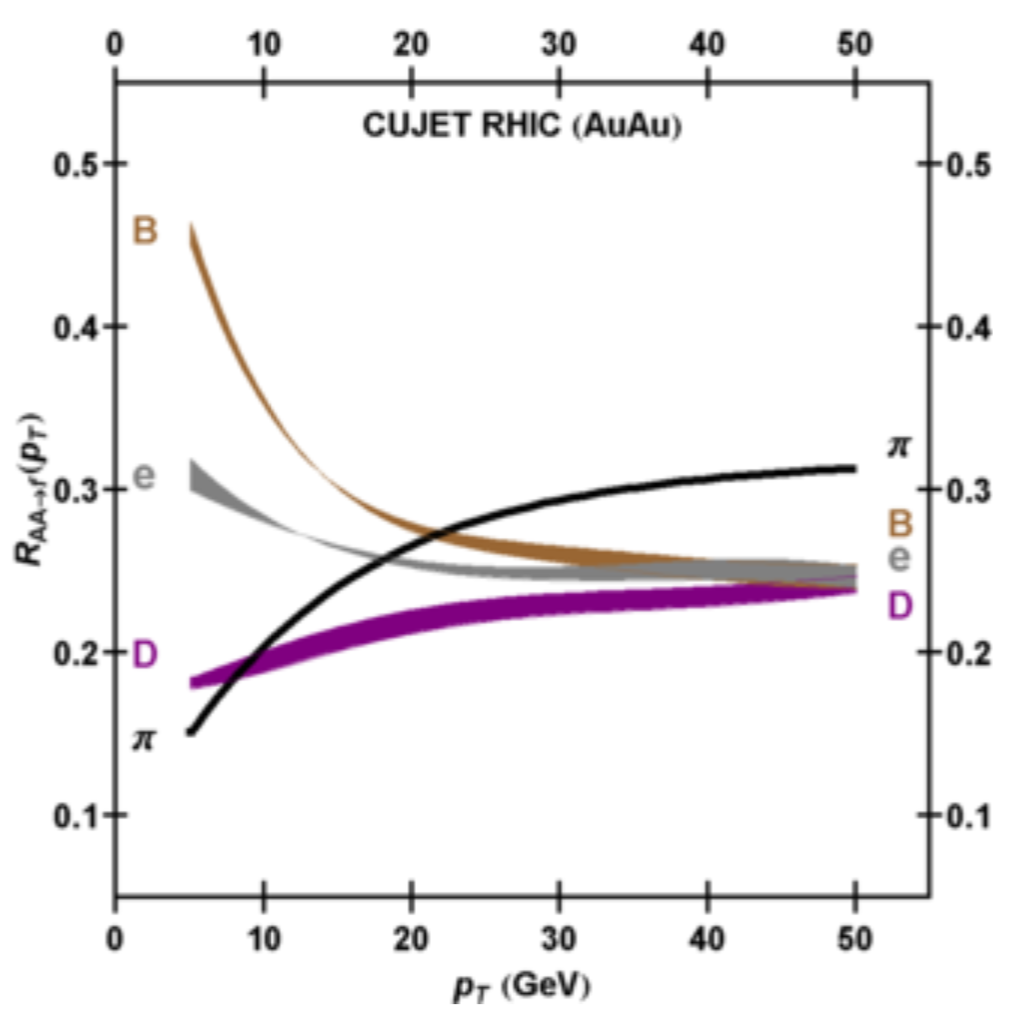
\includegraphics[width=.35\textwidth]{Plots/CUJETRAALHC}
\hspace{1cm}
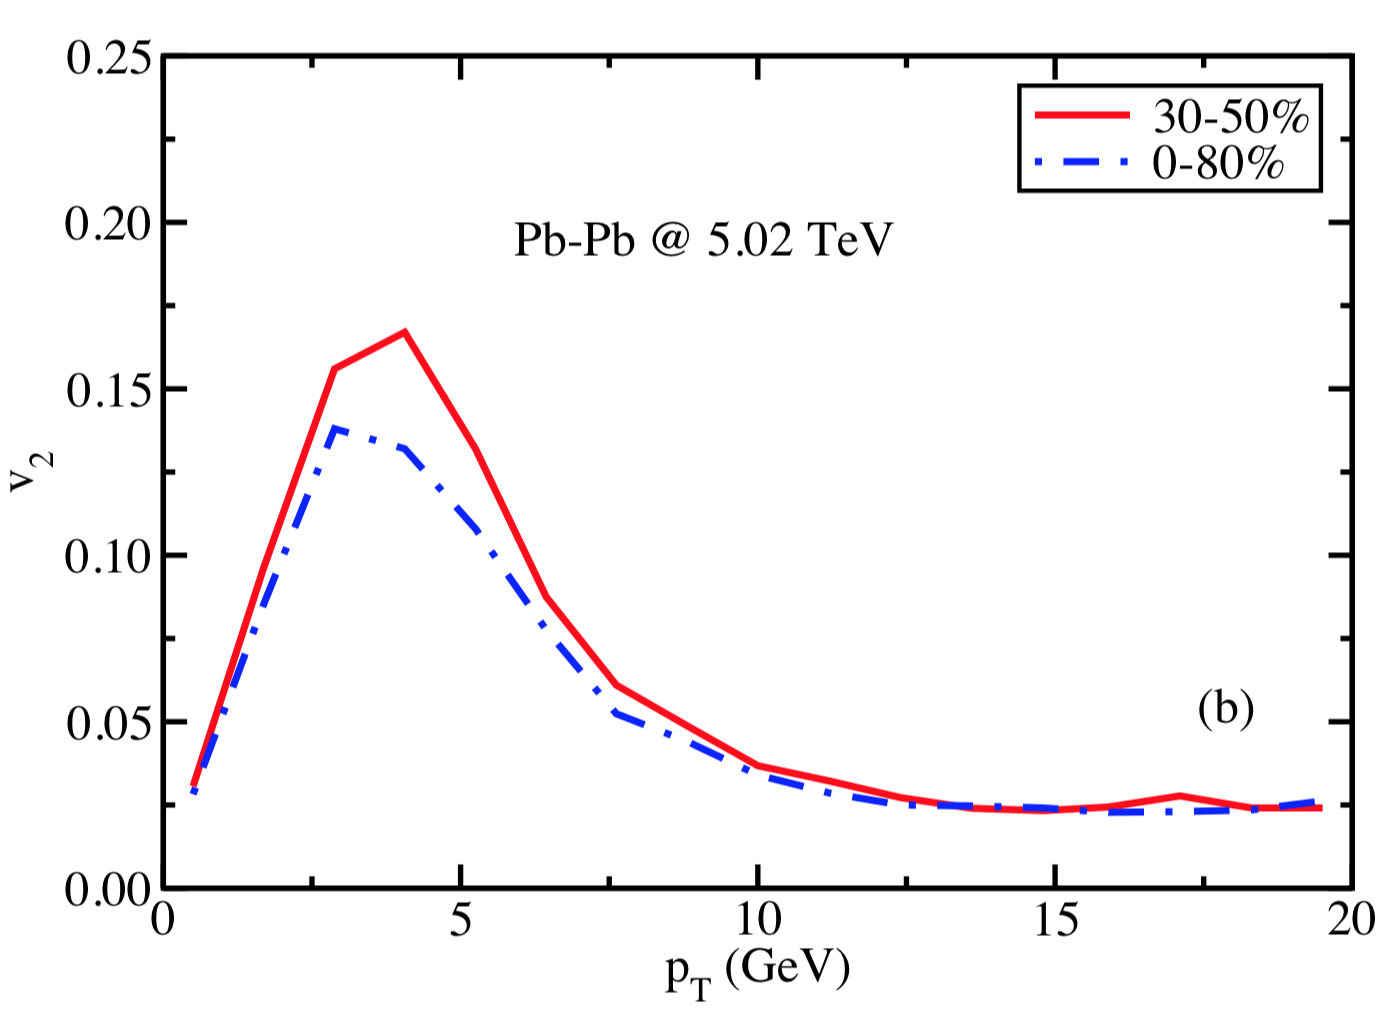
\includegraphics[width=.50\textwidth]{Plots/v2Dmesons_LBT}
\caption{Please write your figure caption here}
\label{theory}       % Give a unique label
\end{figure}

\begin{figure}[ht]
\centering
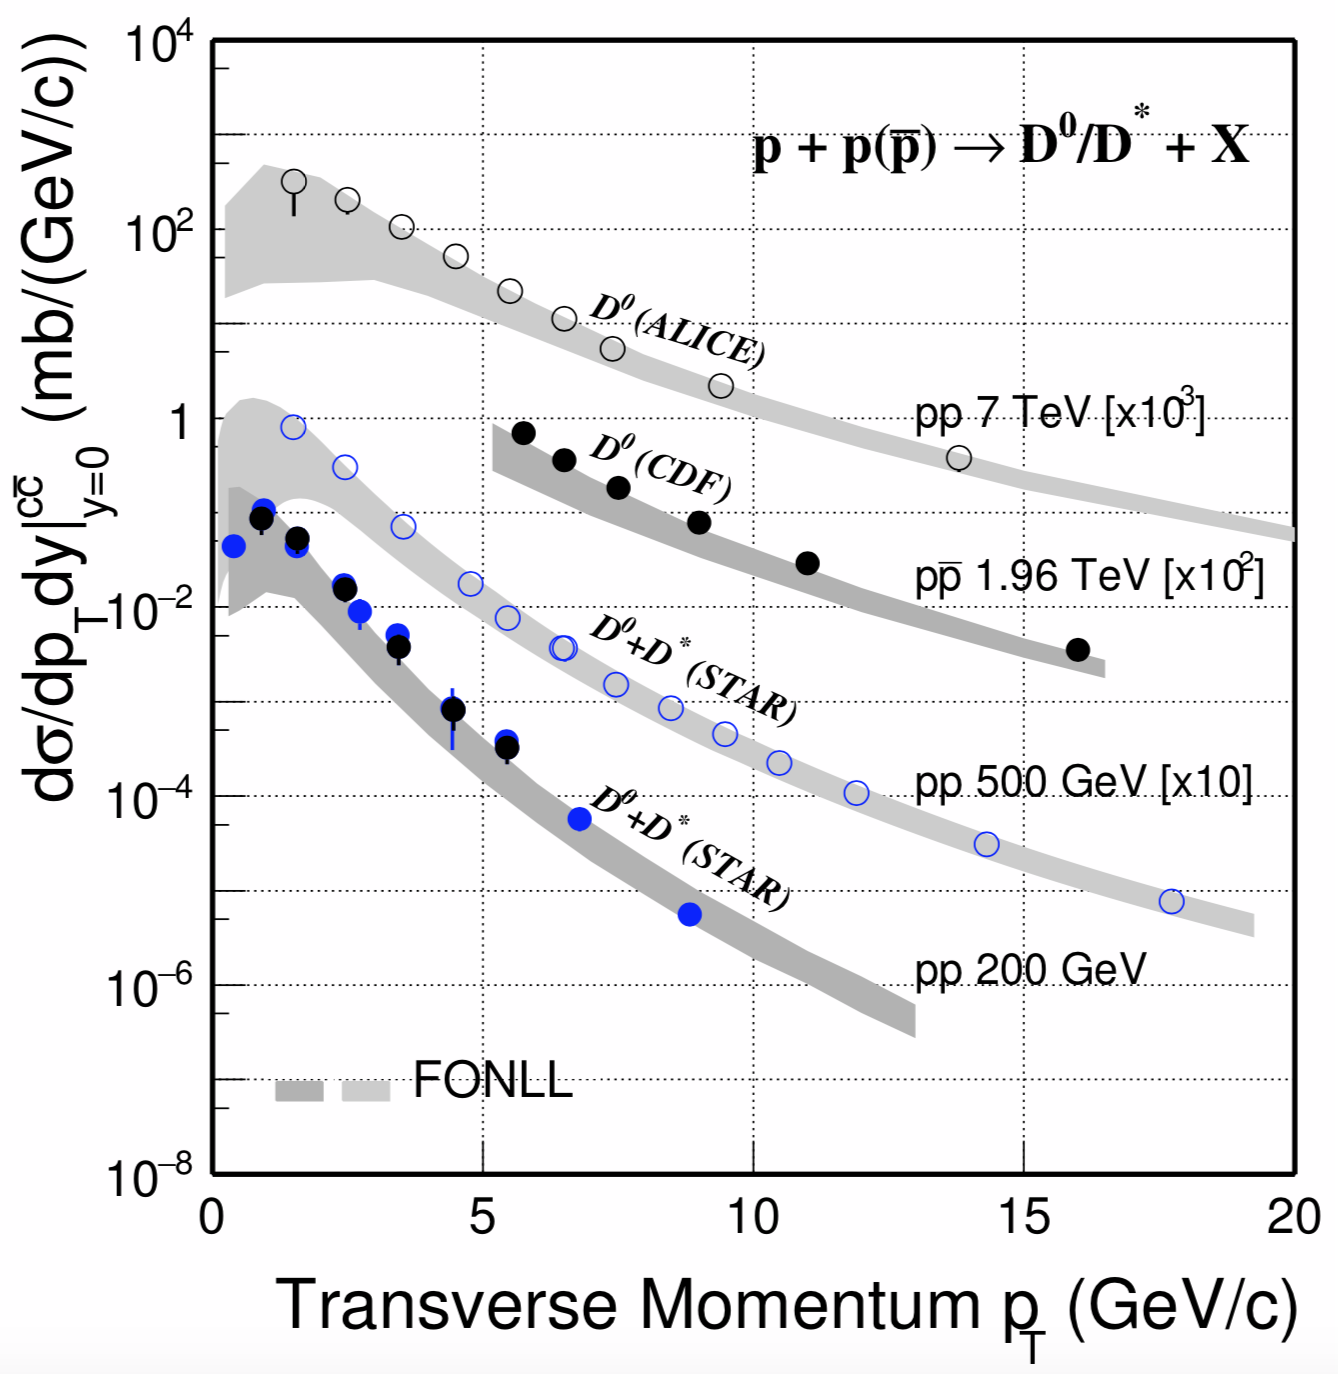
\includegraphics[width=.45\textwidth]{Plots/Dcross_sectionLHCRHIC}
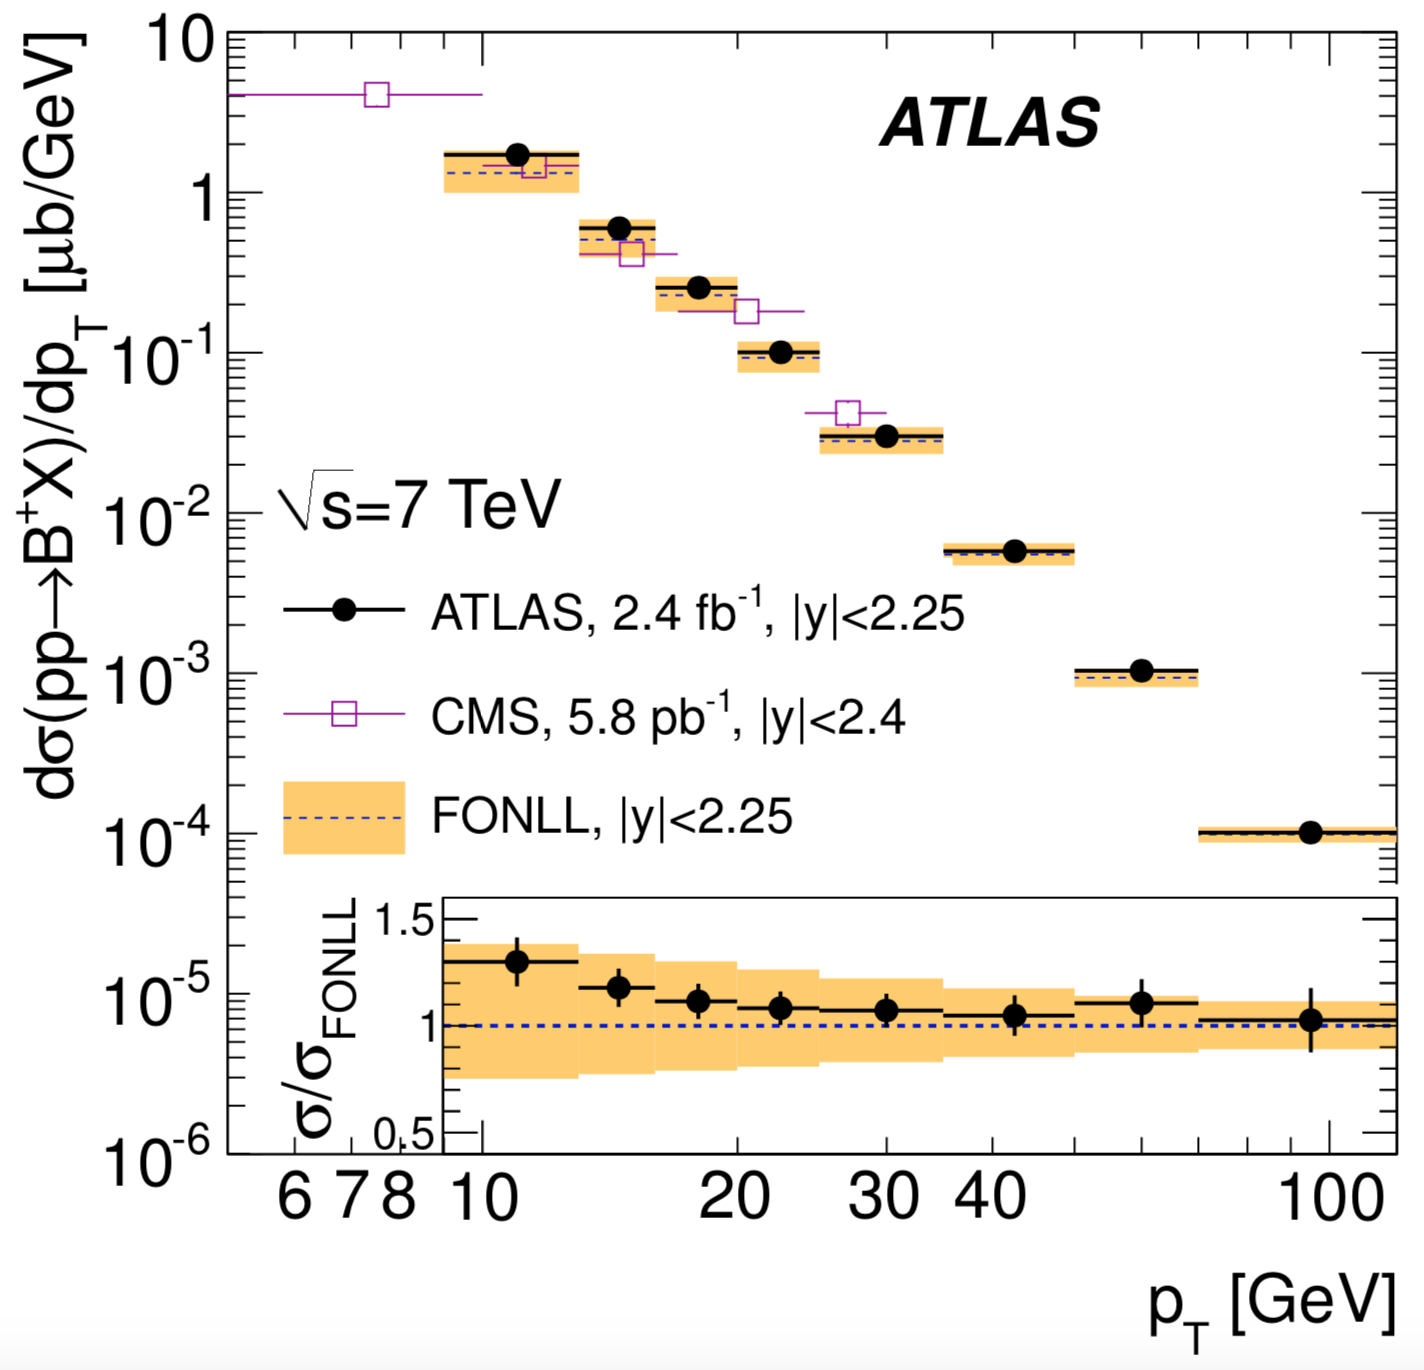
\includegraphics[width=.45\textwidth]{Plots/BplusATLASpp}
\caption{Please write your figure caption here}
\label{ppresults}     
\end{figure}

\begin{figure}[ht]
\centering
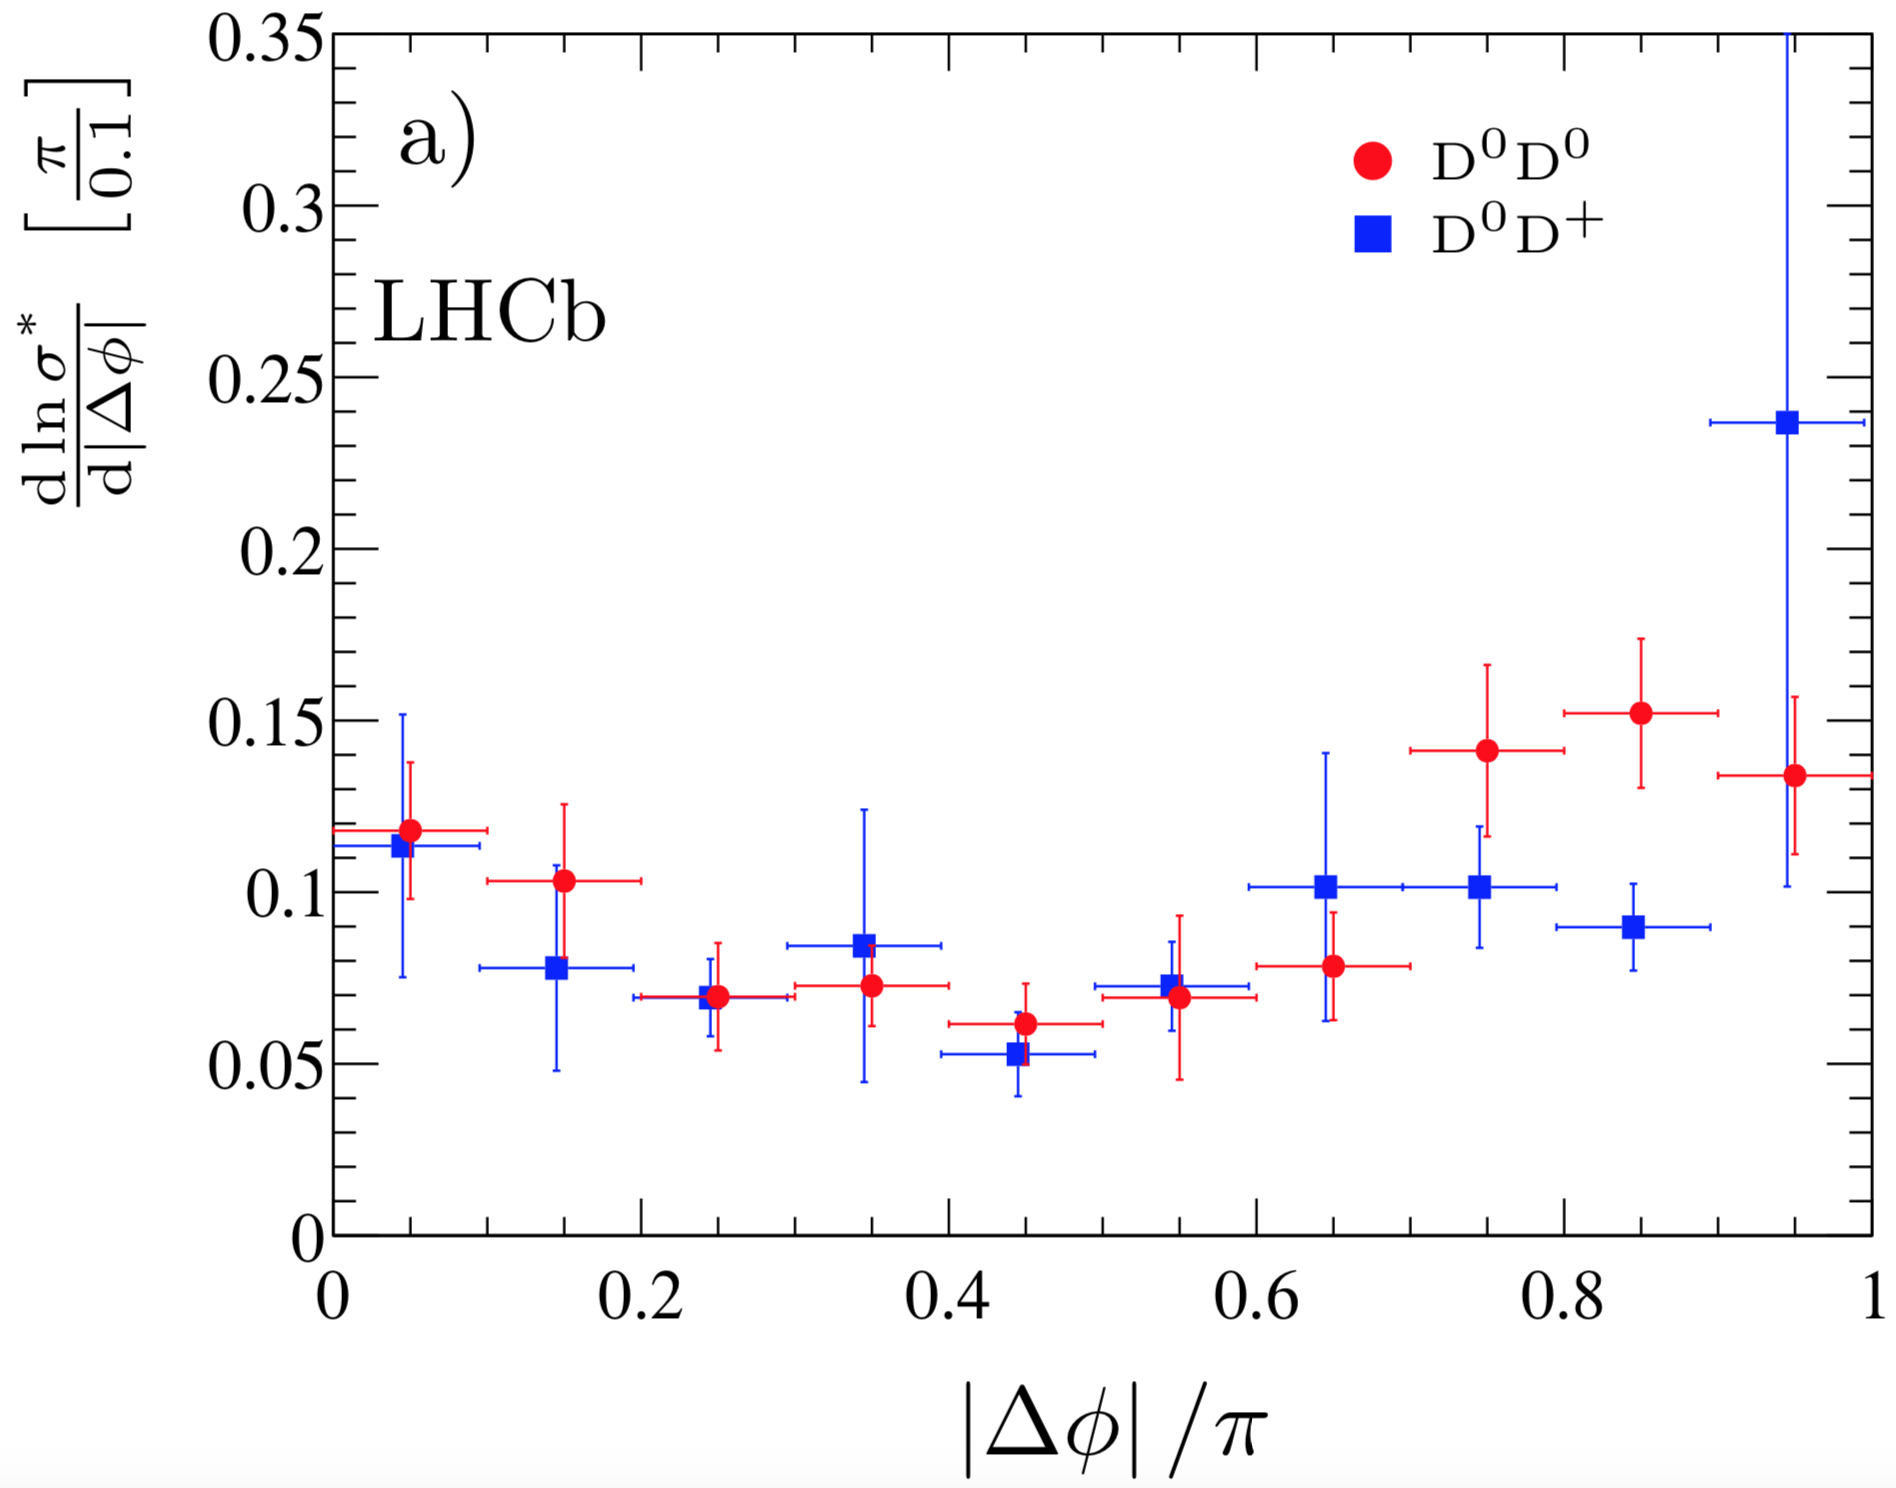
\includegraphics[width=.45\textwidth]{Plots/D0D0ppLHCb}
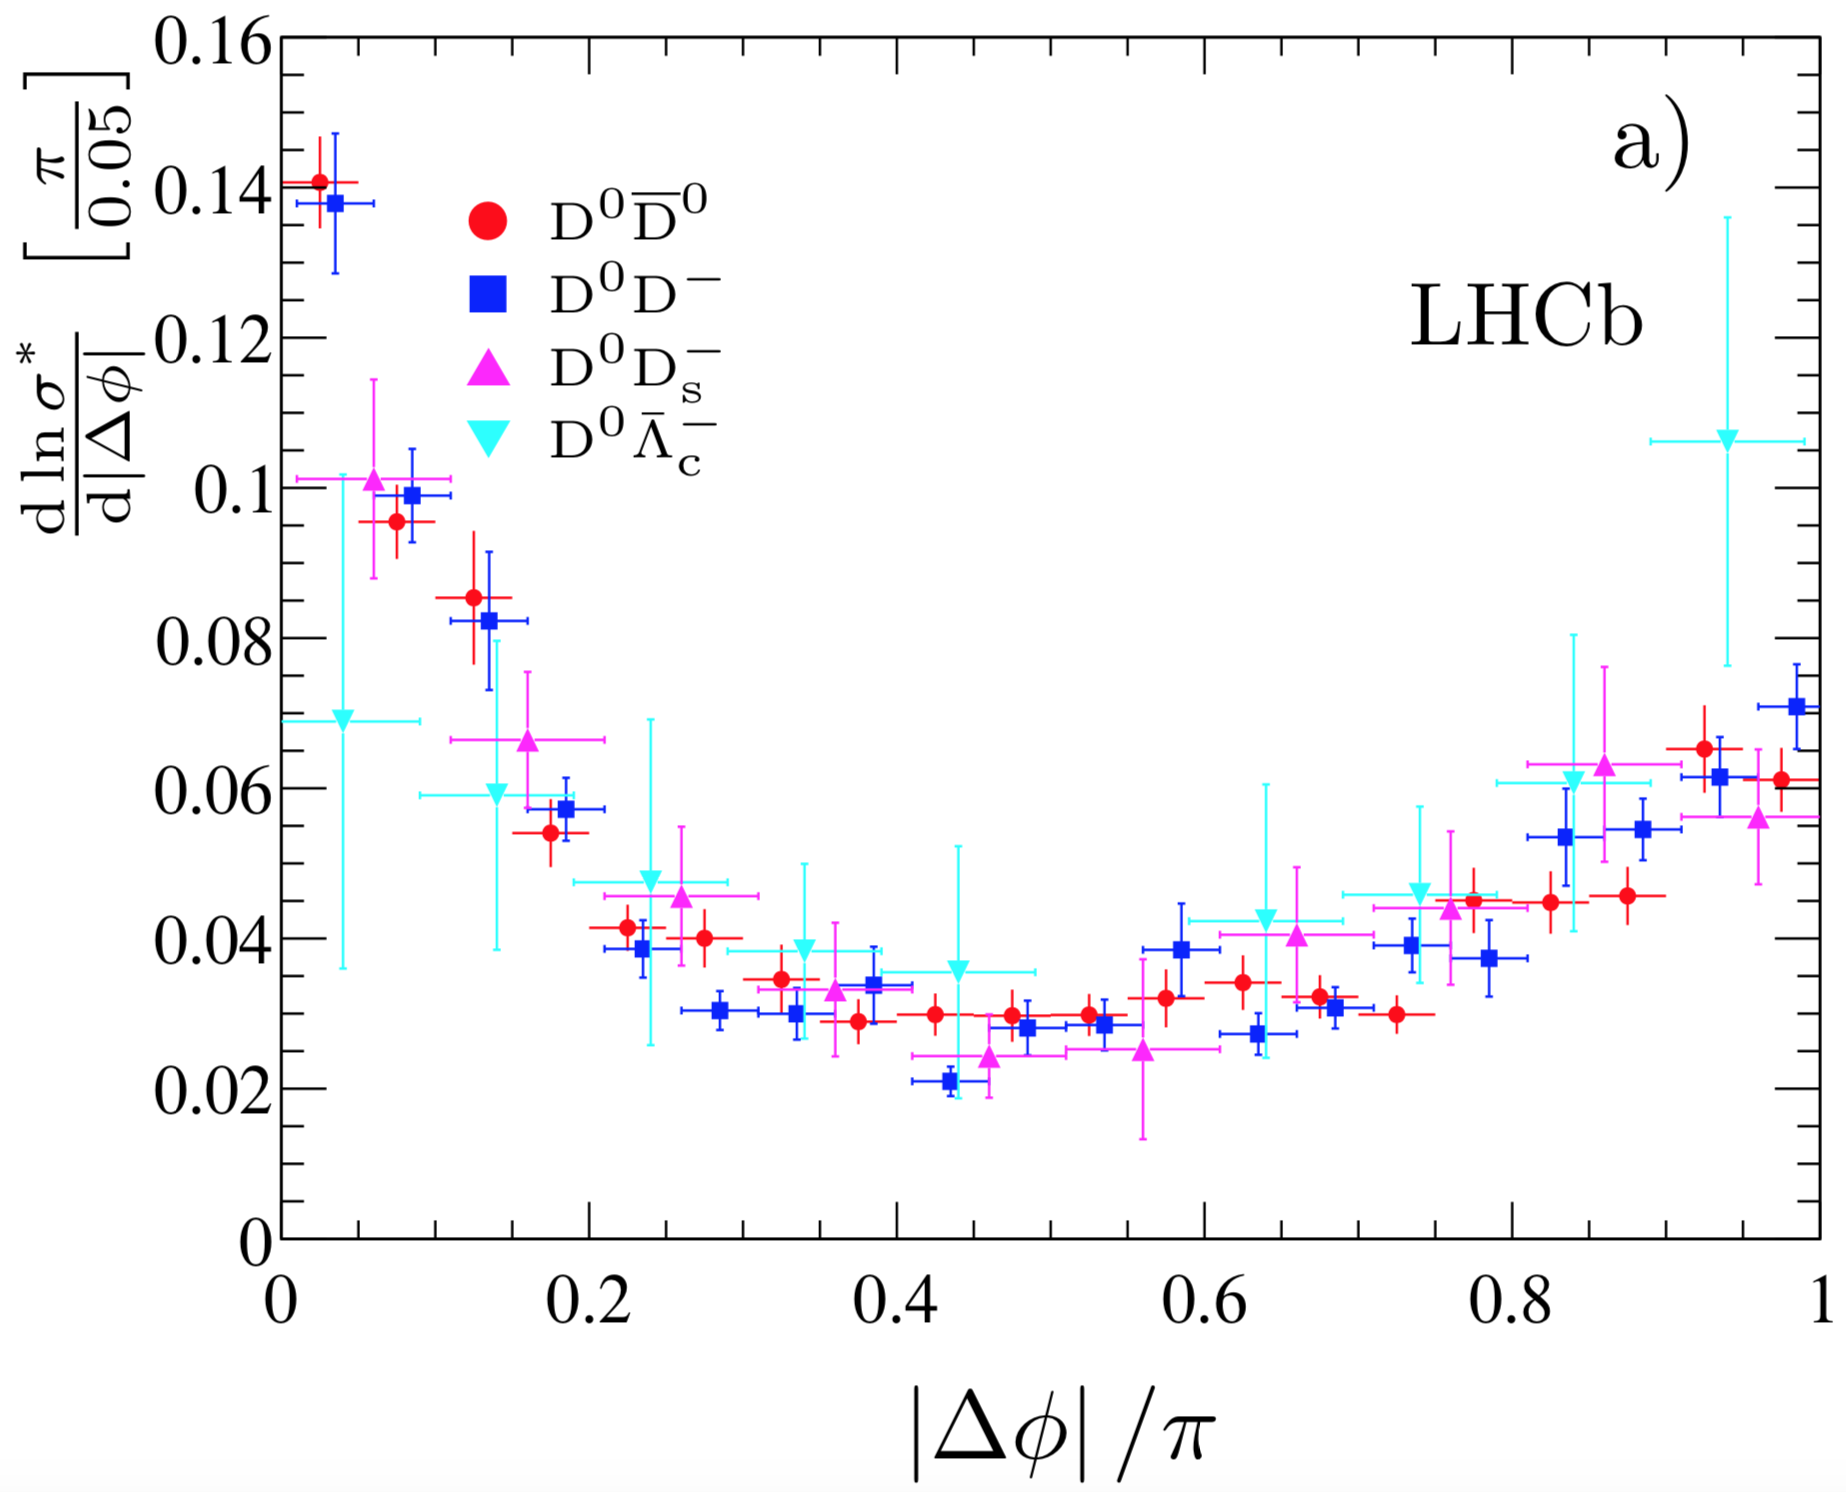
\includegraphics[width=.45\textwidth]{Plots/D0D0barLHCb}
\caption{Please write your figure caption here}
\label{DDbar}     
\end{figure}

\begin{figure}[ht]
\centering
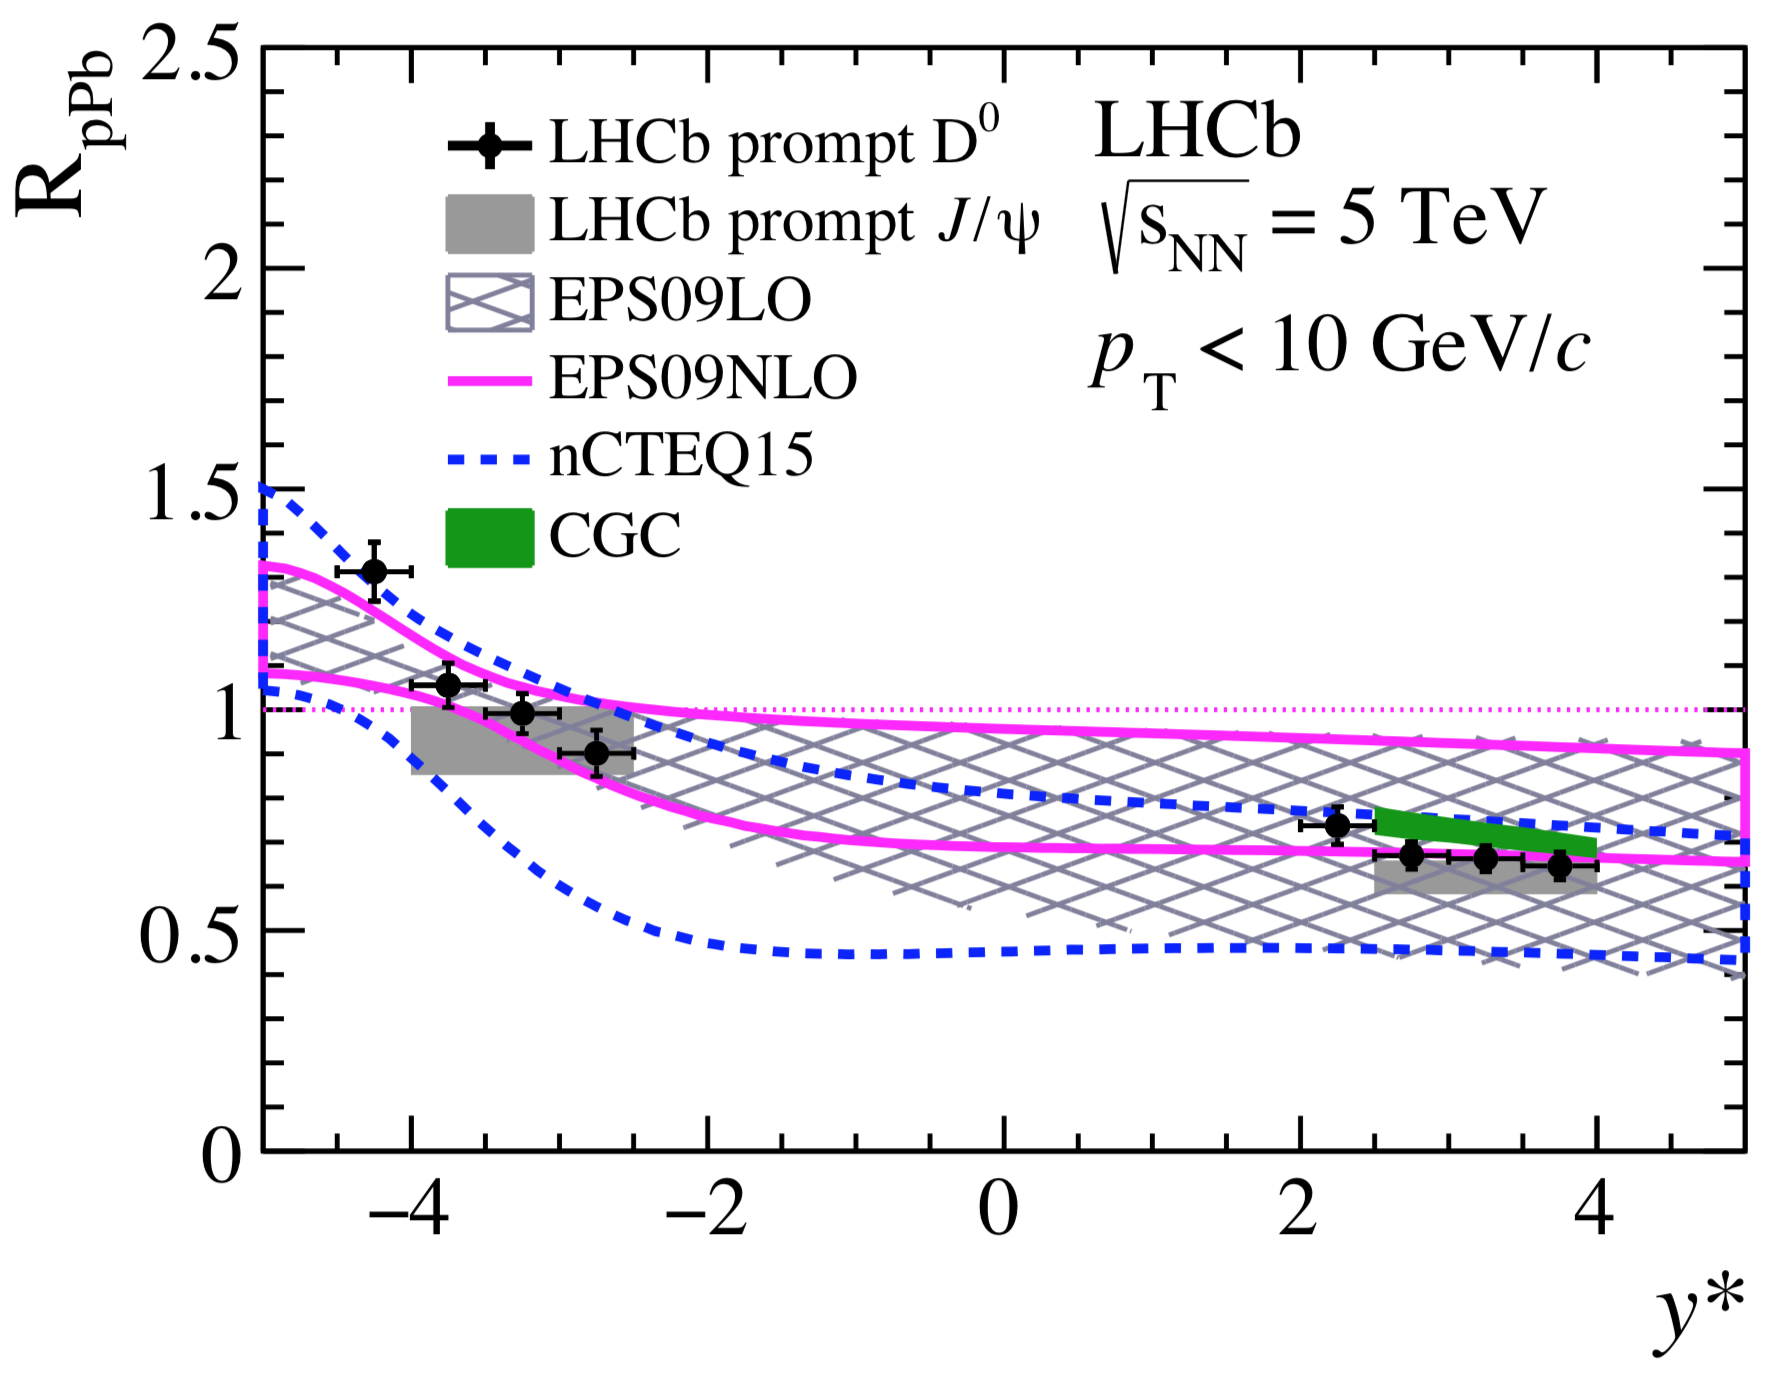
\includegraphics[width=.45\textwidth]{Plots/DRpALHCb2017}
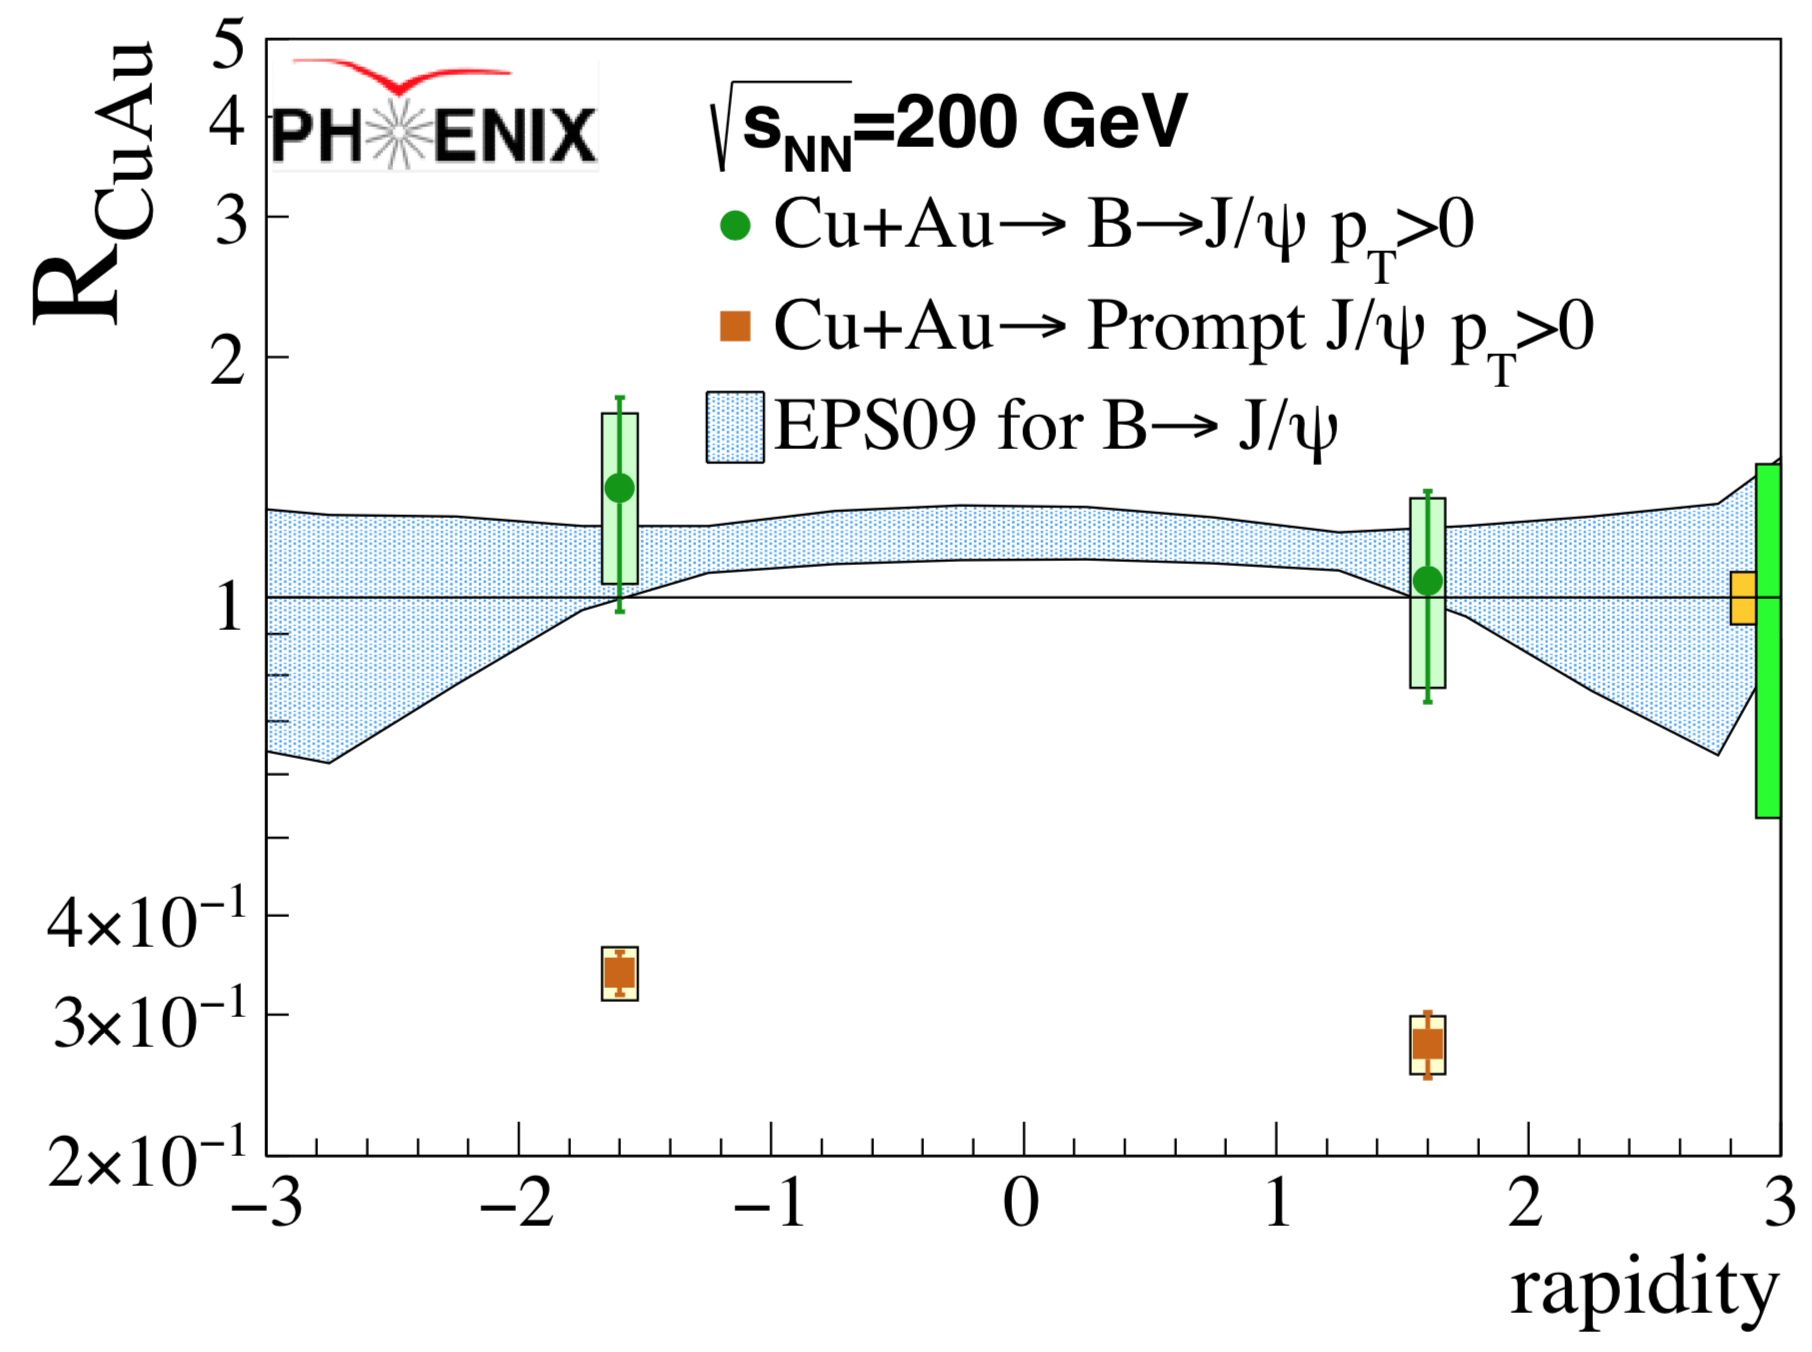
\includegraphics[width=.45\textwidth]{Plots/BRpAPHENIX}
\caption{Please write your figure caption here}
\label{RpA}     
\end{figure}

\begin{figure}[ht]
\centering
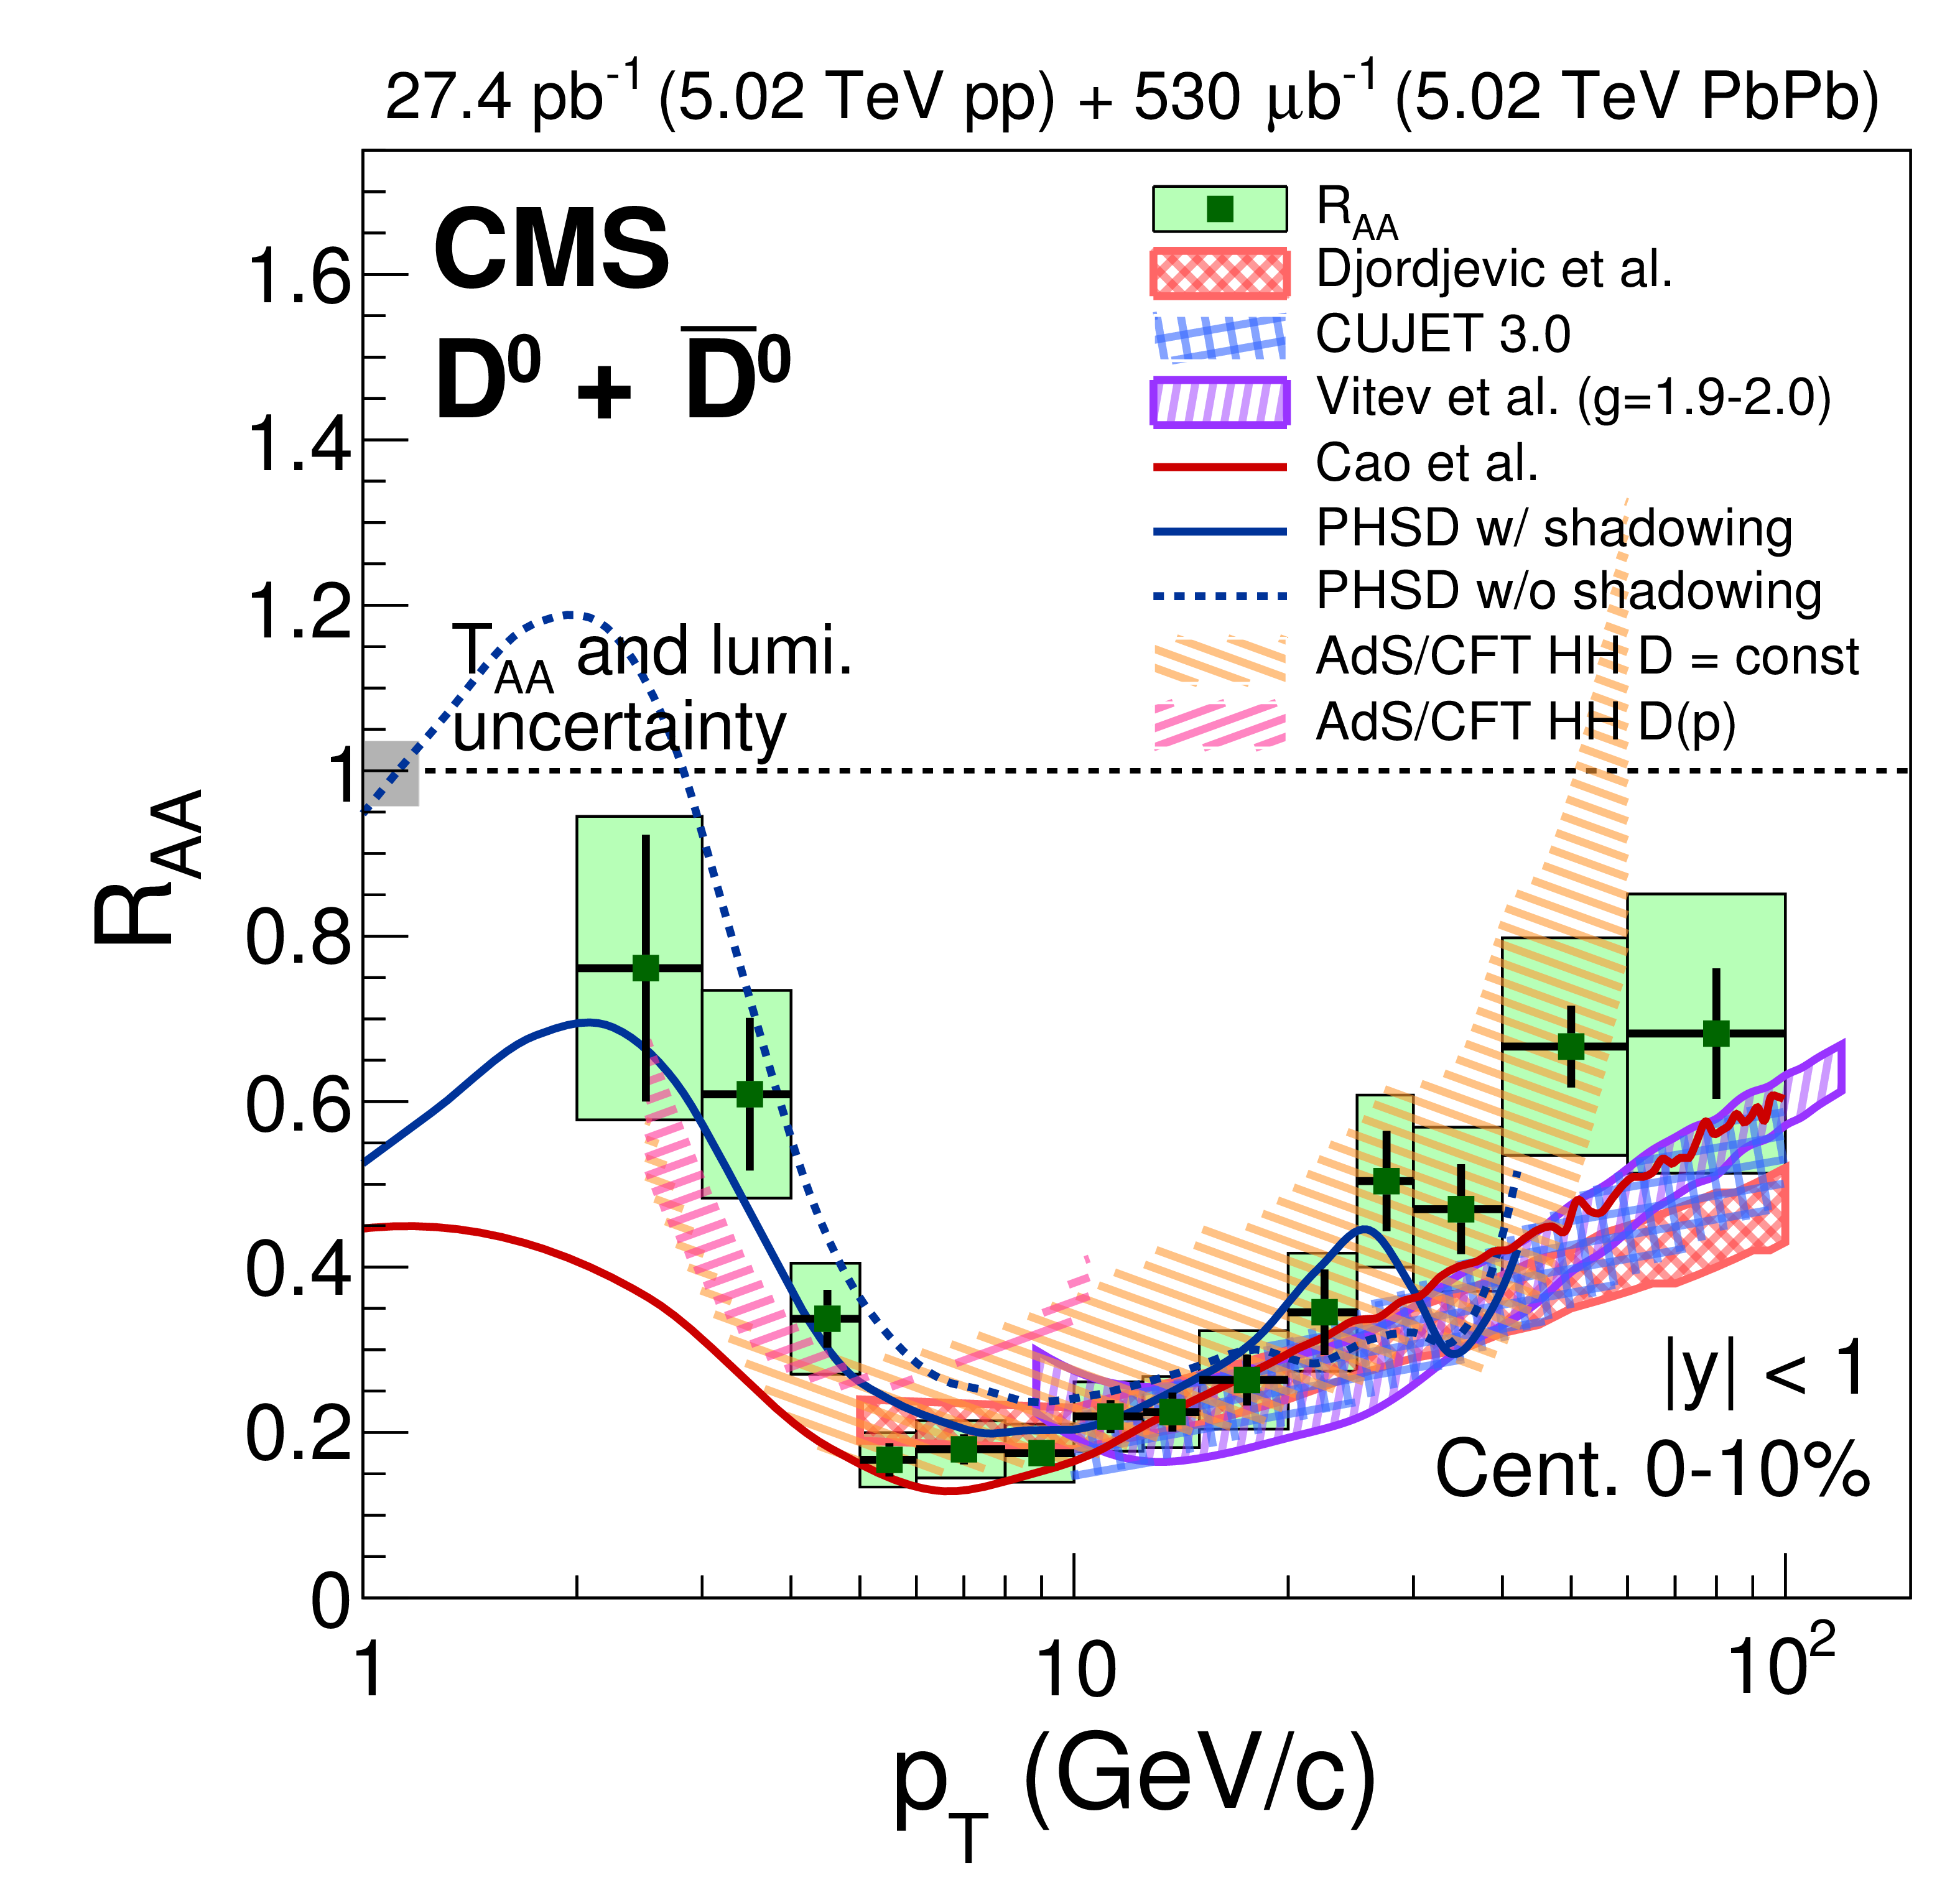
\includegraphics[width=.45\textwidth]{Plots/DRAACMS010}
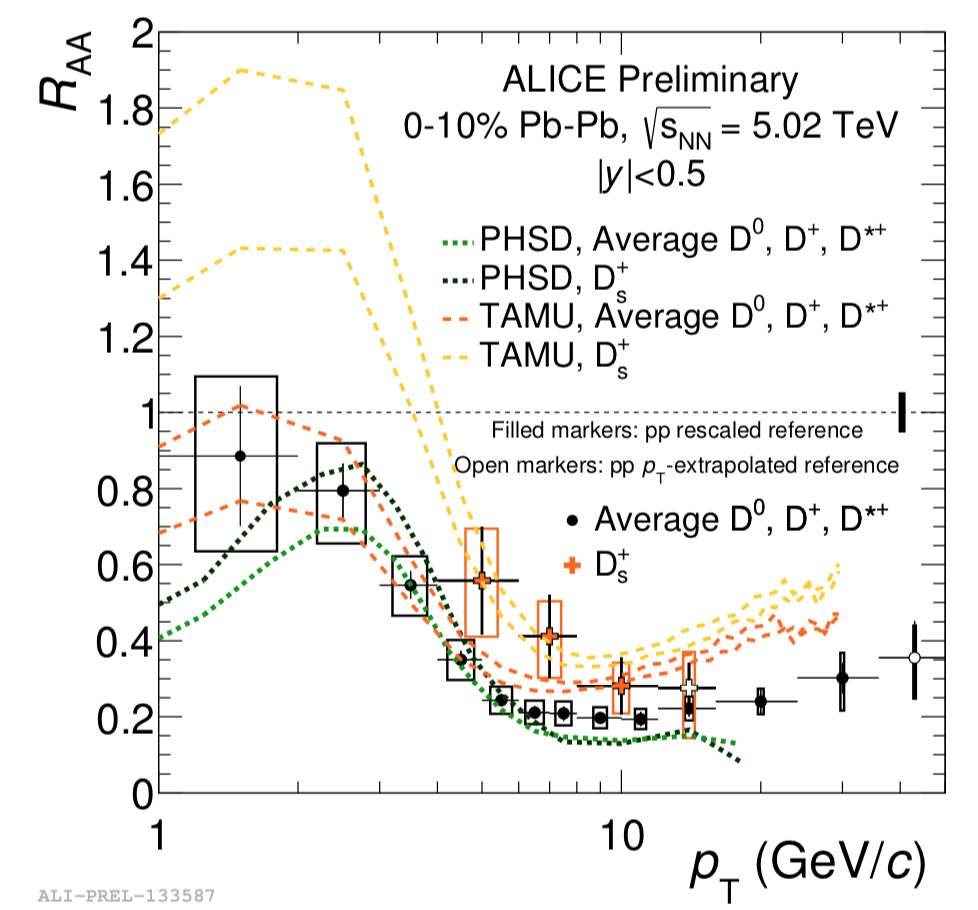
\includegraphics[width=.45\textwidth]{Plots/DmesonRAAALICE2017zoom}
\caption{Please write your figure caption here}
\label{DRAA}     
\end{figure}

\begin{figure}[ht]
\centering
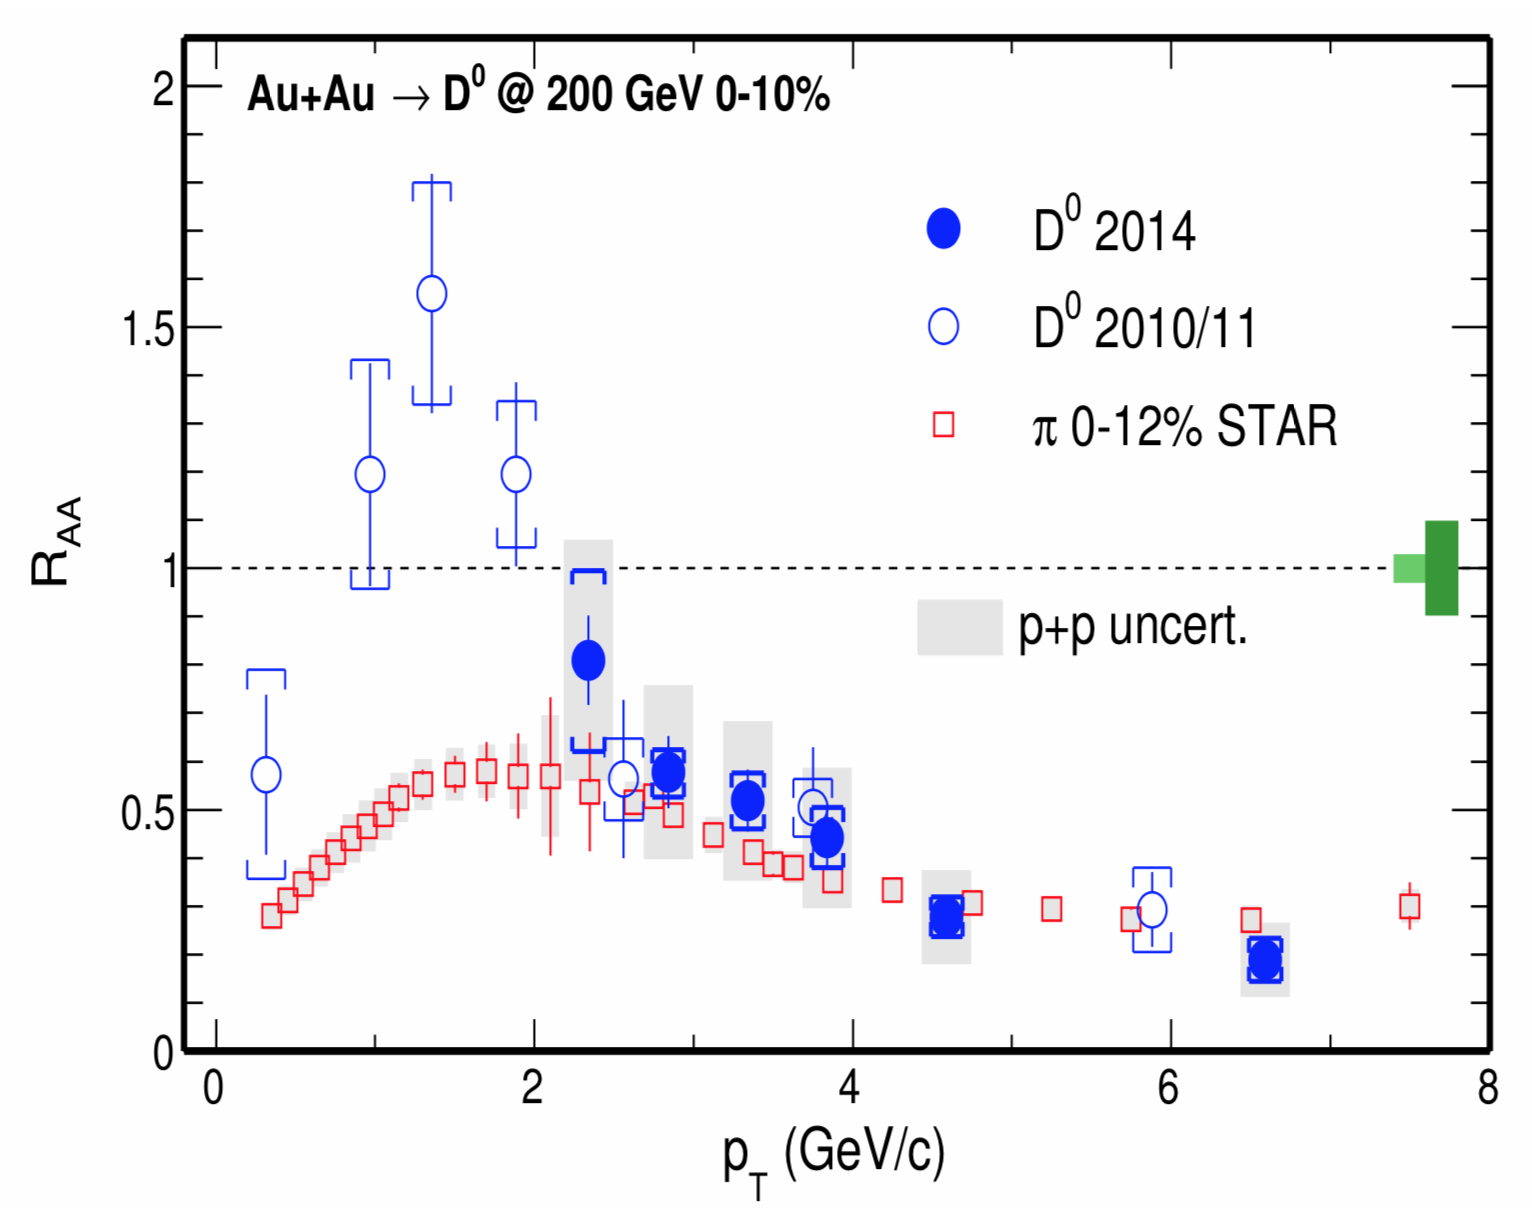
\includegraphics[width=.45\textwidth]{Plots/DRAASTARAuAu}
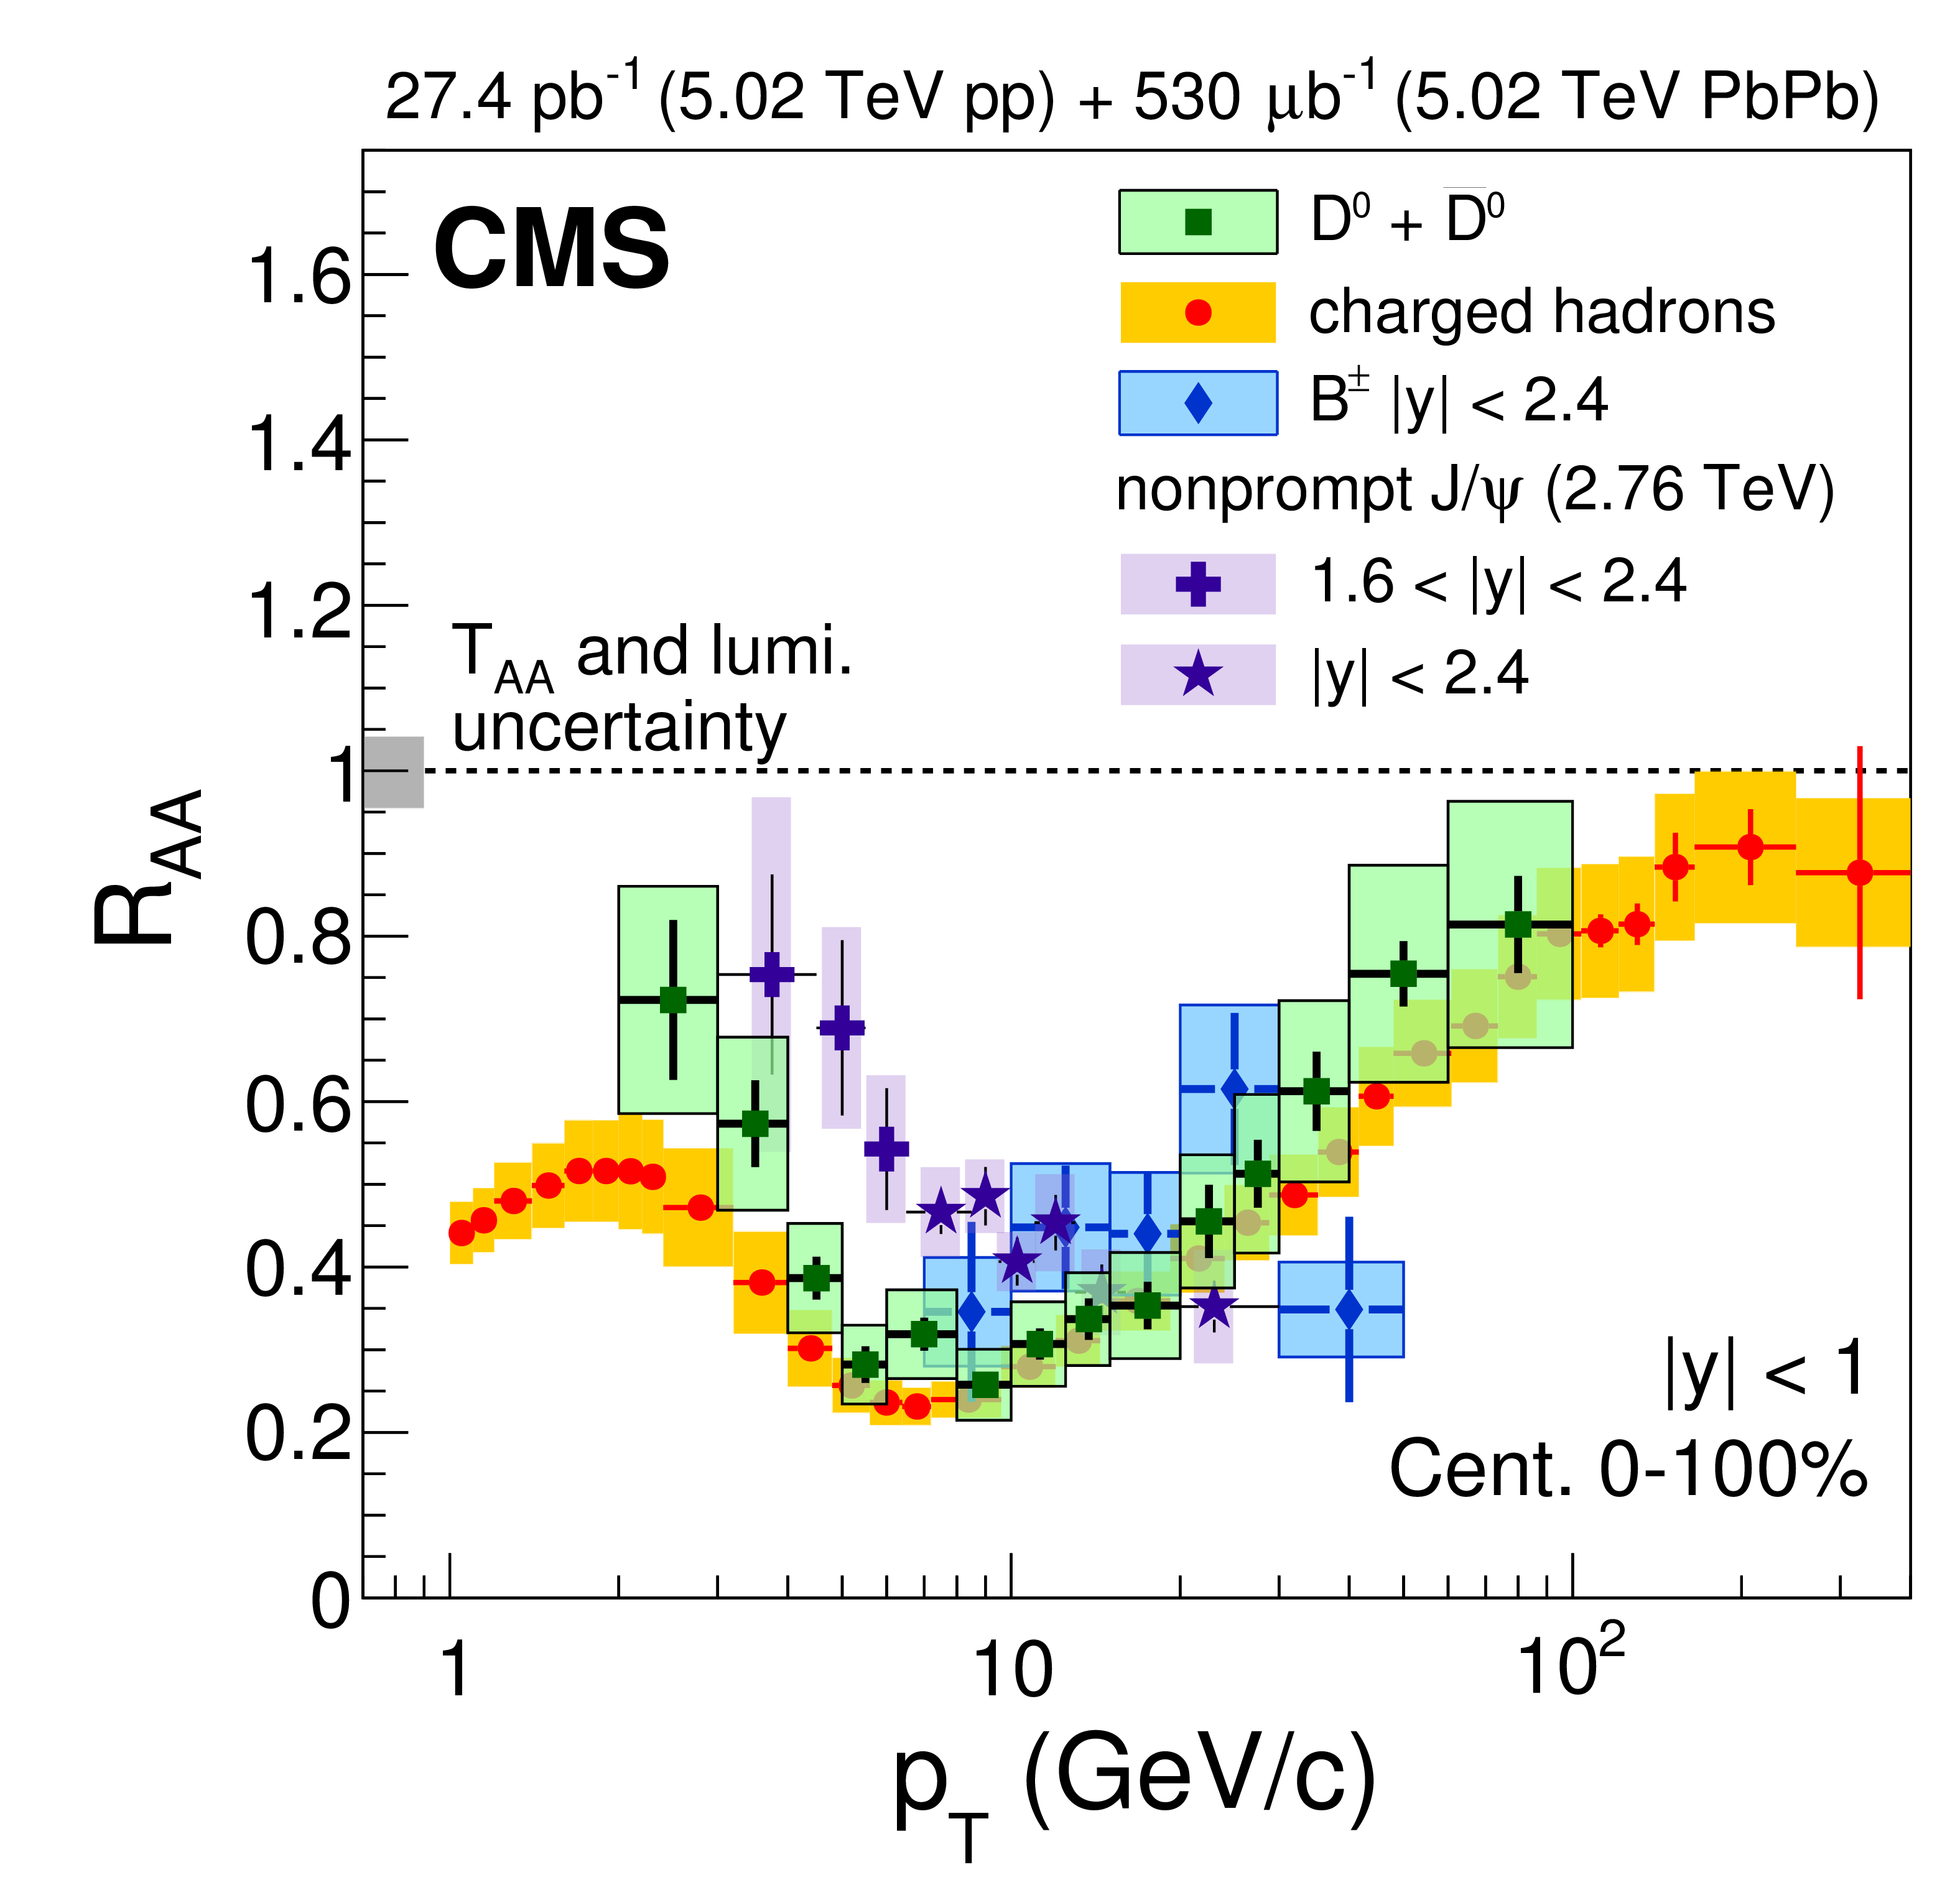
\includegraphics[width=.45\textwidth]{Plots/DBNonPromptRAACMS}
\caption{Please write your figure caption here}
\label{FlavourRAA}     
\end{figure}

\begin{figure}[ht]
\centering
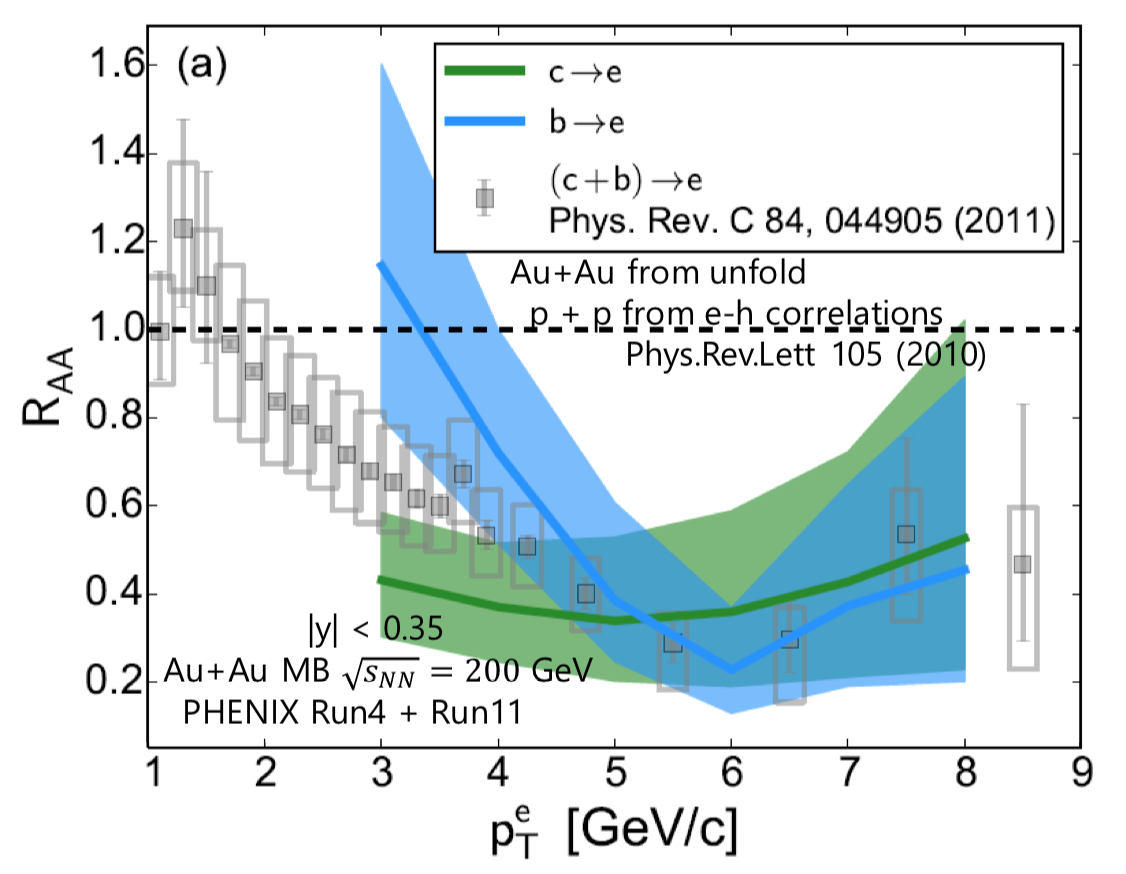
\includegraphics[width=.95\textwidth]{Plots/BPHENIXAuAu}
\caption{Please write your figure caption here}
\label{FlavourRAAPHENIX}
\end{figure}

\begin{figure}[ht]
\centering
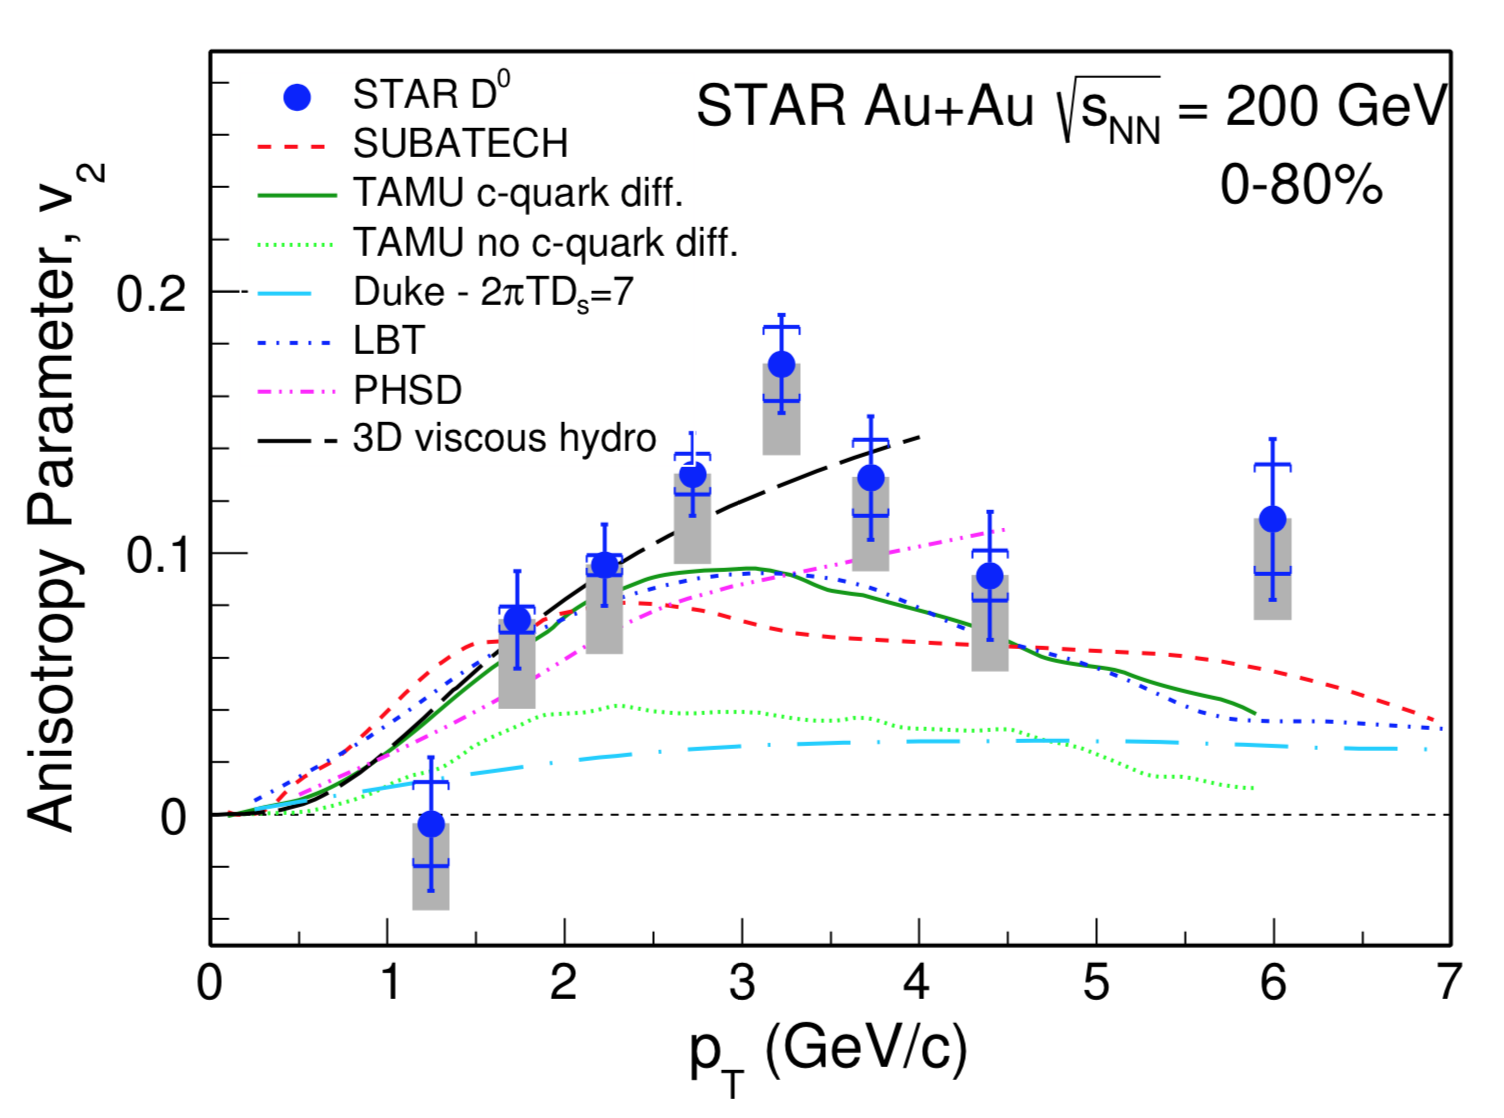
\includegraphics[width=.40\textwidth]{Plots/Dmesonv2STAR}
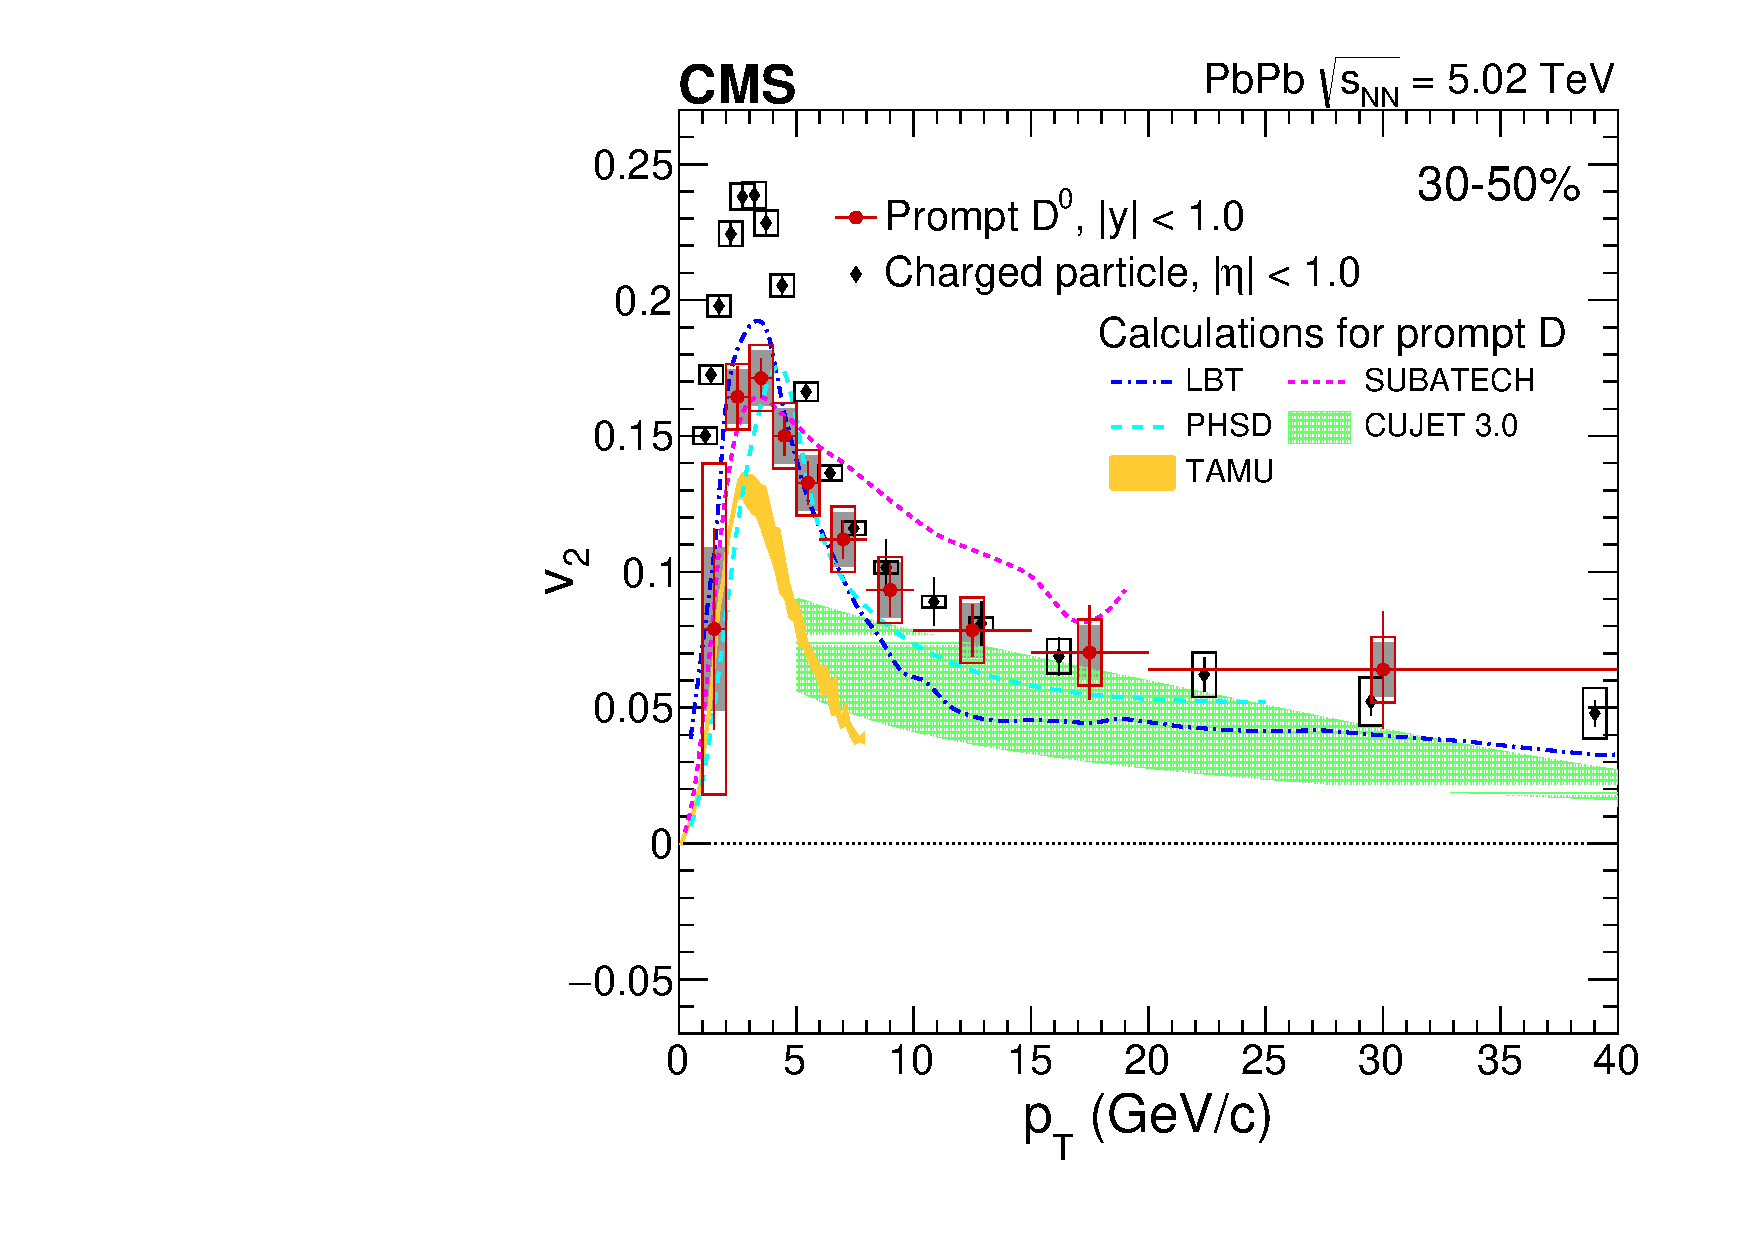
\includegraphics[width=.29\textwidth]{Plots/Dv2CMS3050.pdf}
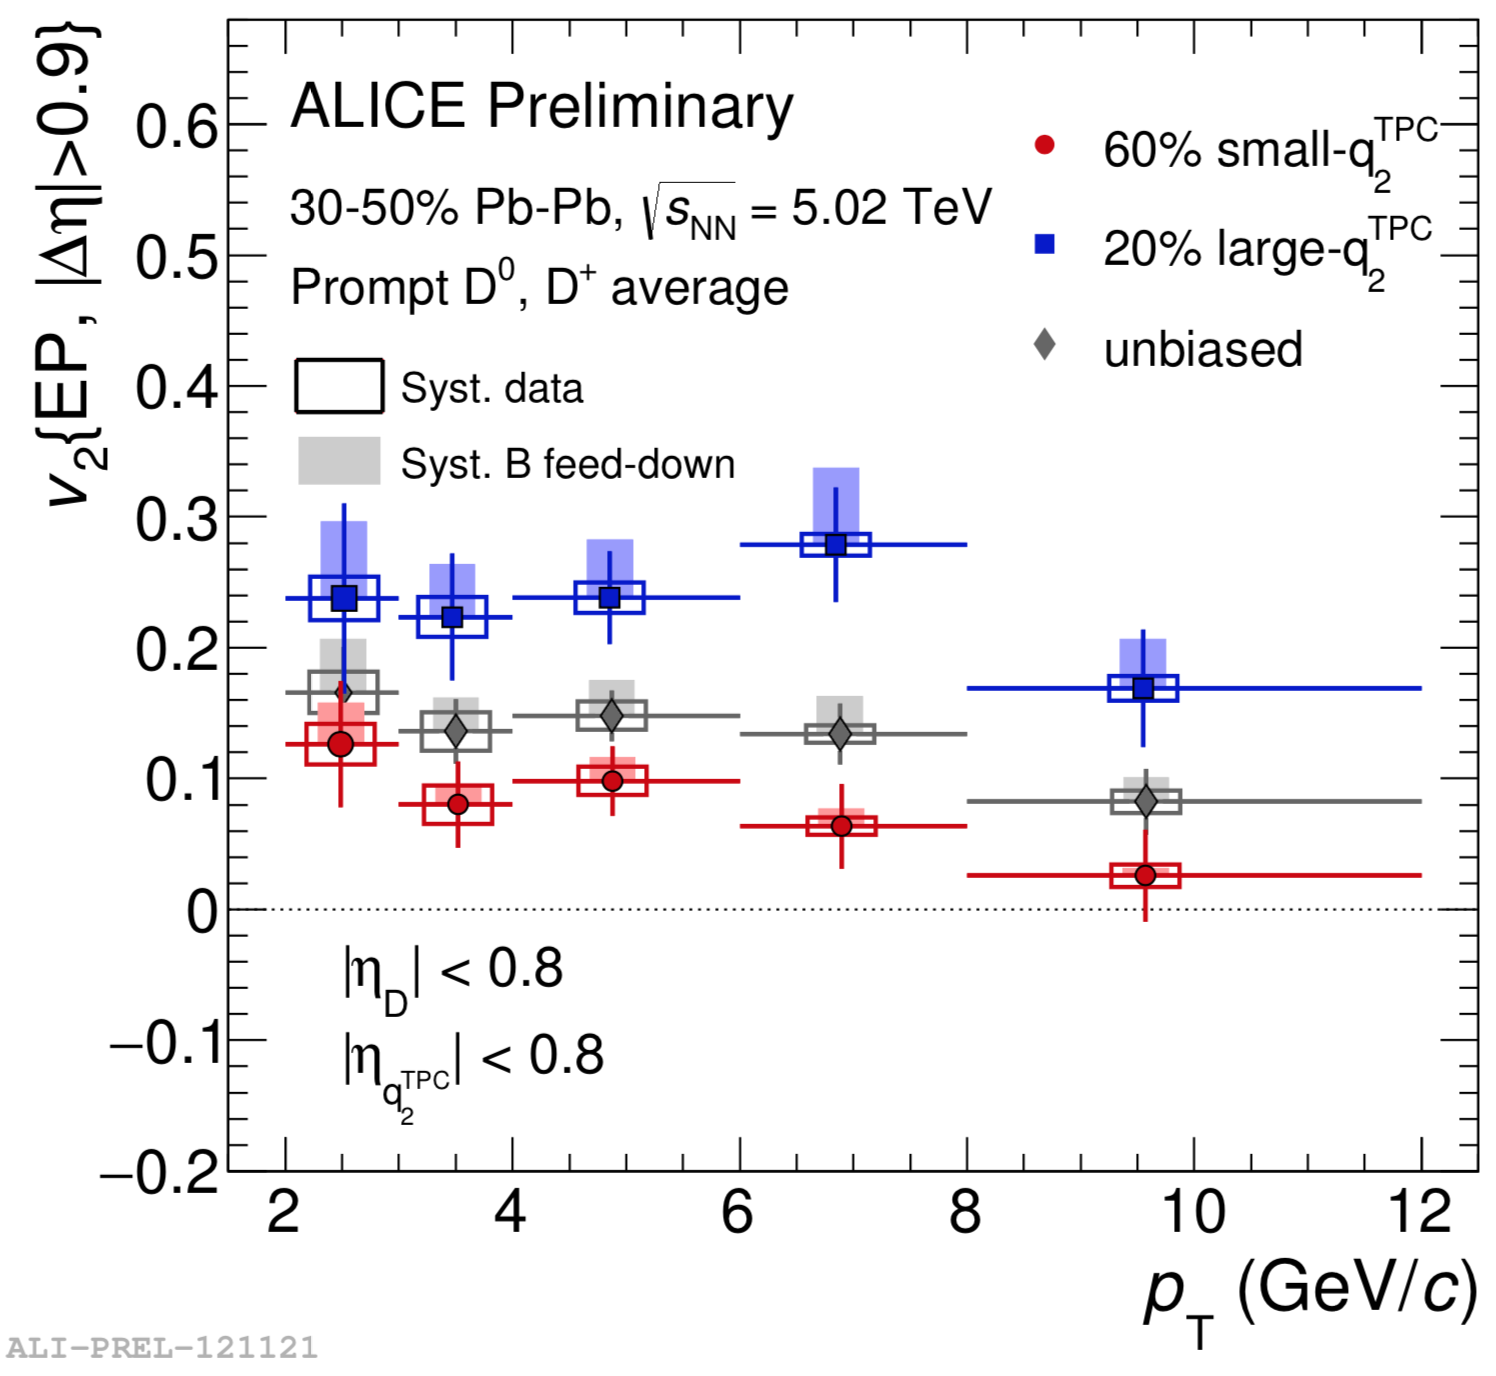
\includegraphics[width=.29\textwidth]{Plots/DmesonEventShapeALICEPbPb}
\caption{Please write your figure caption here}
\label{Dvn}     
\end{figure}

\begin{figure}[ht]
\centering
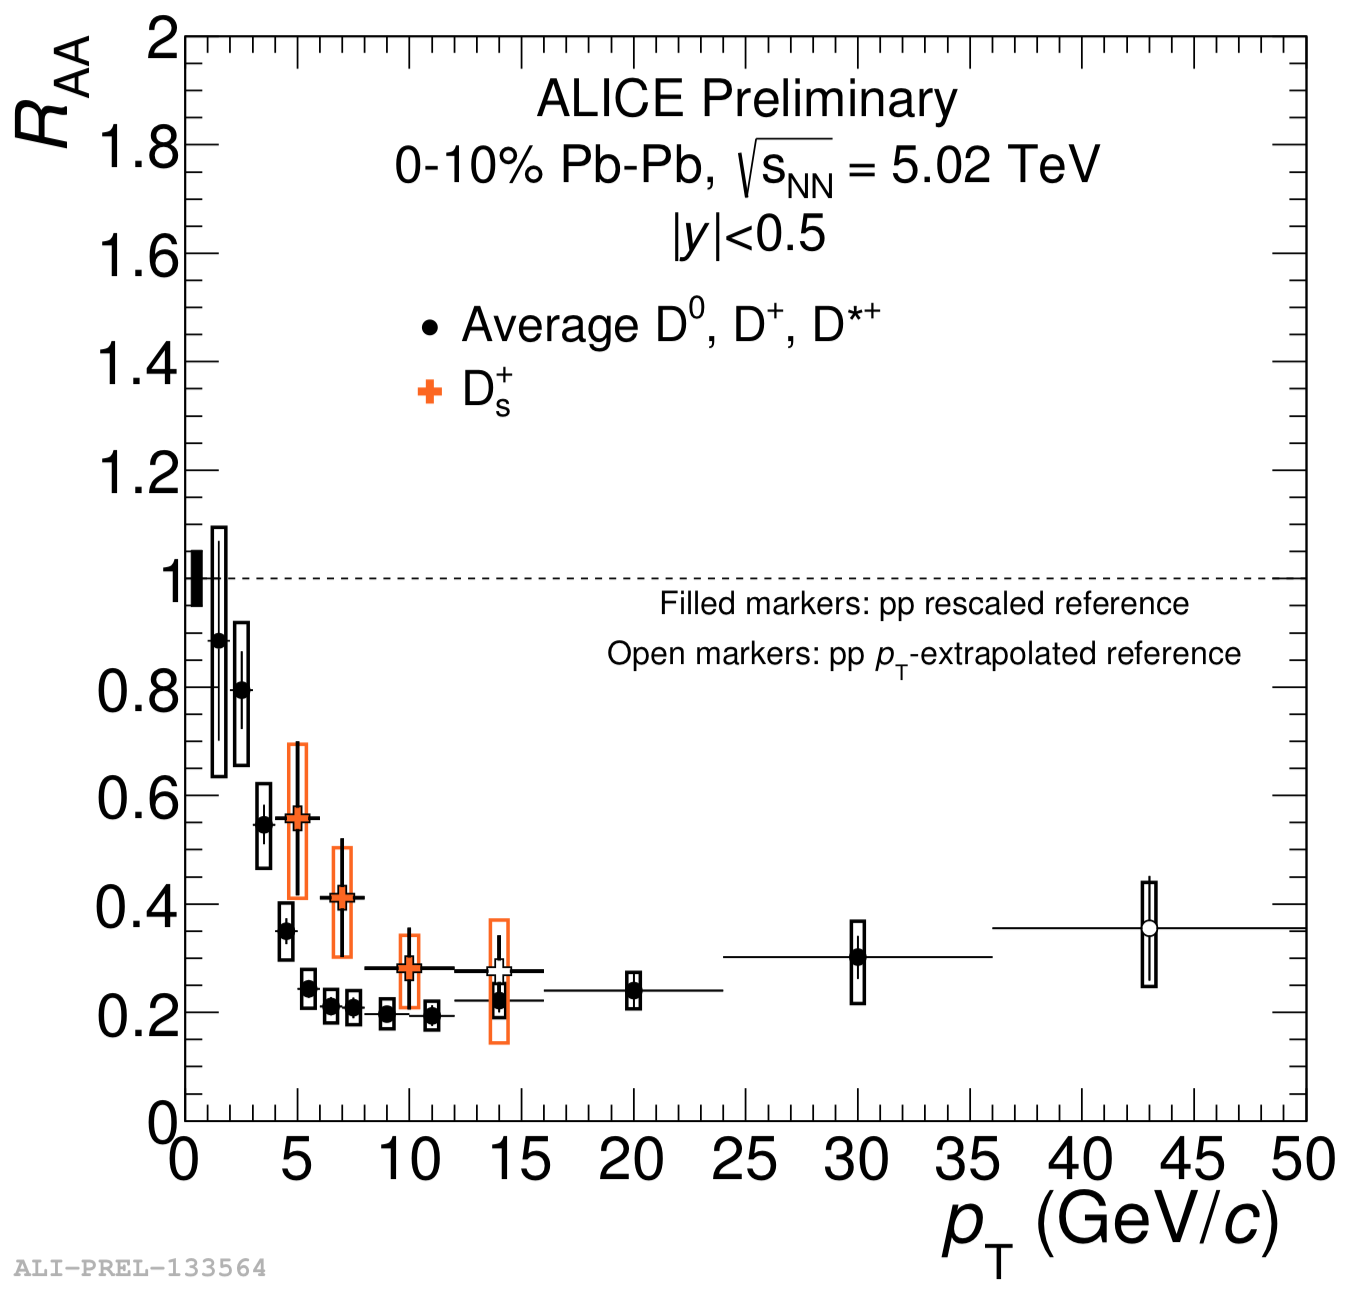
\includegraphics[width=.45\textwidth]{Plots/DsDRAA502TeV}
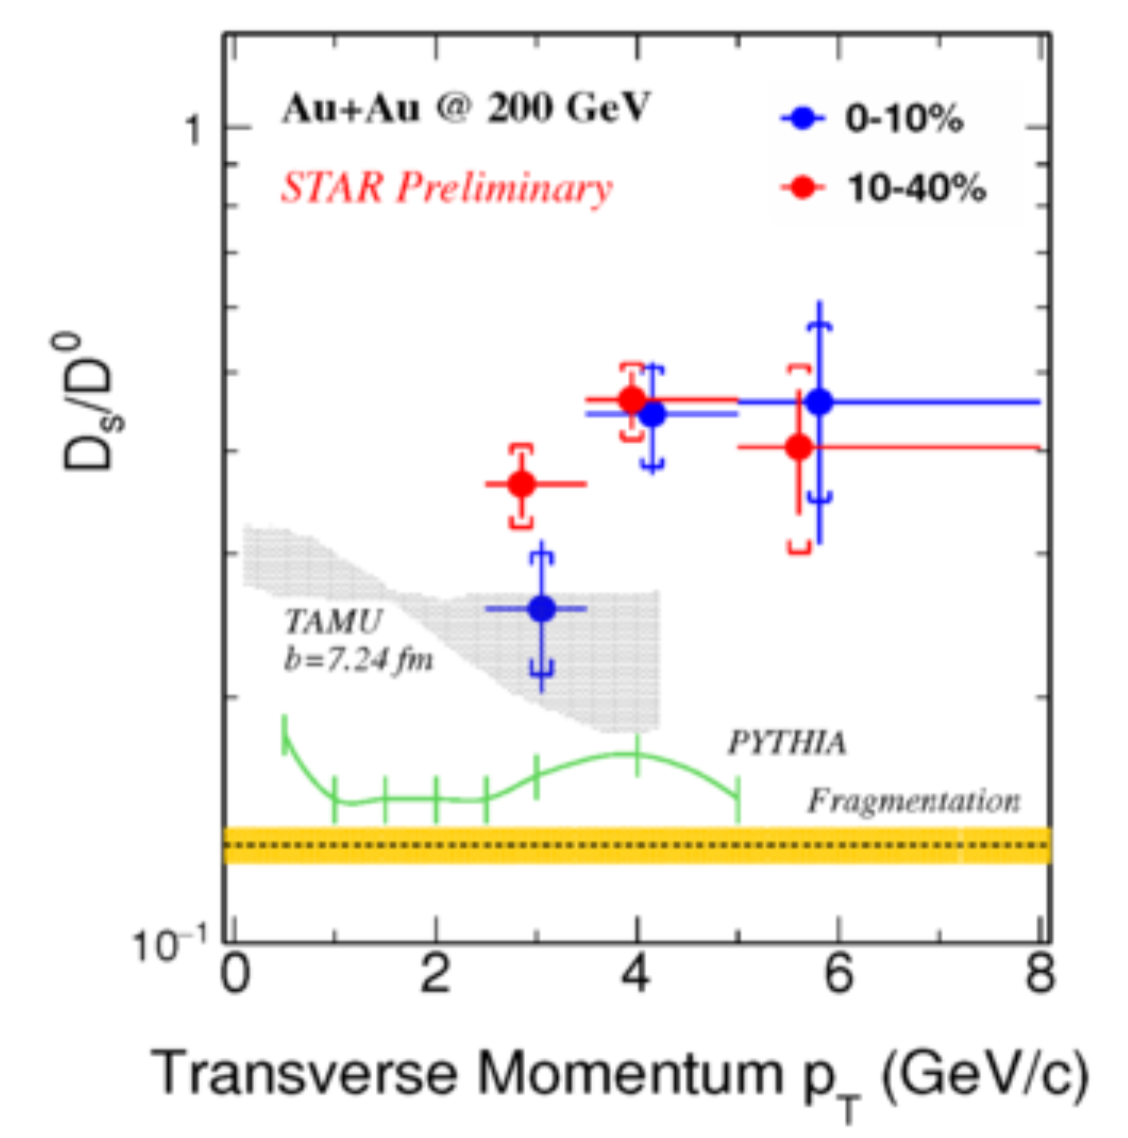
\includegraphics[width=.45\textwidth]{Plots/DsDSTARAuAu}
\caption{Please write your figure caption here}
\label{recombinationMesons}     
\end{figure}

\begin{figure}[ht]
\centering
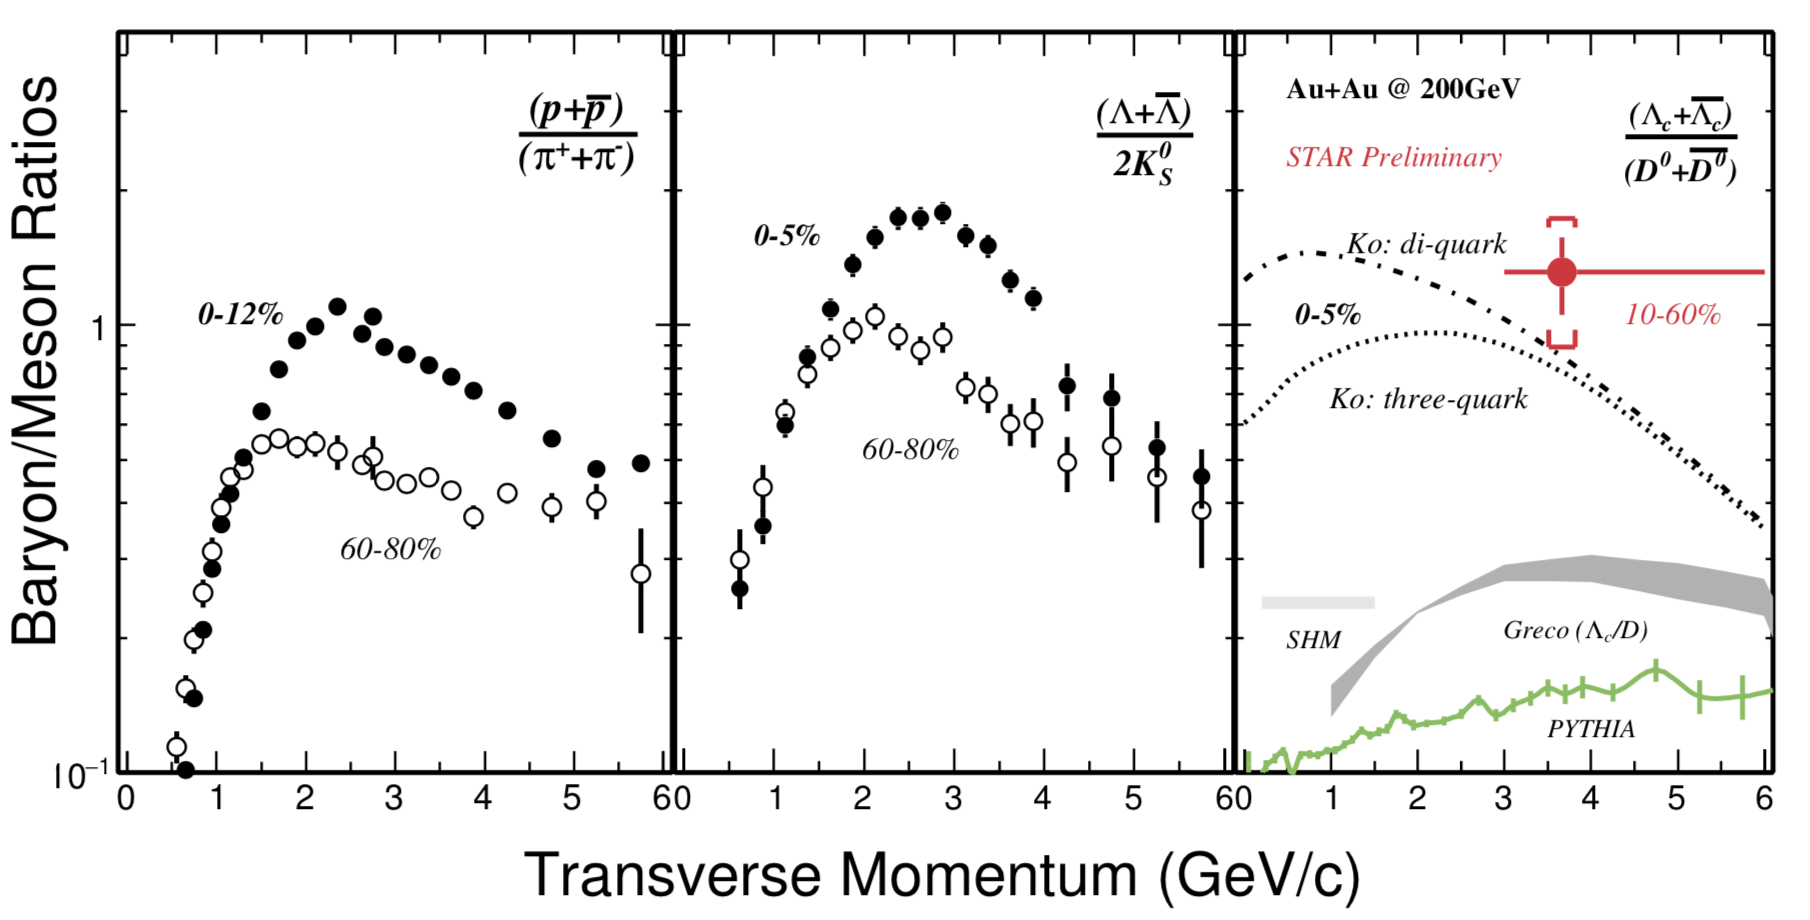
\includegraphics[width=.90\textwidth]{Plots/LambdacSTARAuAu}
\caption{Please write your figure caption here}
\label{recombinationBaryons}     
\end{figure}


%%%%%%%%%%%%%%%%%%%%%%%%%
\begin{thebibliography}{}
\bibitem{RefJ}
Journal Author, Journal \textbf{Volume}, page numbers (year)
% Format for books
%\bibitem{RefB}
%Book Author, \textit{Book title} (Publisher, place, year) page numbers
% etc
\end{thebibliography}
\end{document}

% end of file template.tex

%<div id='footer'><table width='100%'><tr><td class='right'><a href='http://fusioninventory.org/'><span class='copyright'>FusionInventory 9.1+1.0 | copyleft <img src='/glpi/plugins/fusioninventory/pics/copyleft.png'/>  2010-2016 by FusionInventory Team</span></a></td></tr></table></div>